\documentclass{patmorin}
\usepackage[T1]{fontenc}
\usepackage[utf8]{inputenc}
\usepackage{amsmath}
\usepackage{amsfonts}
\usepackage{amsthm}
\usepackage{graphicx}
\usepackage{enumerate}
\usepackage{amsfonts}
\usepackage{amsthm,mathtools}
\usepackage{pat}
\usepackage{paralist}
\usepackage{stmaryrd}

\usepackage[longnamesfirst,numbers,sort&compress]{natbib}
\usepackage[noabbrev,capitalise]{cleveref}
\allowdisplaybreaks
%\sloppy
%%%%%%%%%%
\makeatletter
\def\NAT@spacechar{~}
\makeatother
%%%%%%%%%%
\crefname{lem}{Lemma}{Lemmas}
\crefname{thm}{Theorem}{Theorems}
\crefname{cor}{Corollary}{Corollaries}
\crefname{conj}{Conjecture}{Conjectures}
\crefname{obs}{Observation}{Observations}
\crefname{prop}{Proposition}{Propositions}
\crefname{clm}{Claim}{Claims}
\crefname{openproblem}{Open Problem}{Open Problems}
\crefformat{equation}{(#2#1#3)}
\Crefformat{equation}{Equation #2(#1)#3}

\setlength{\parskip}{1ex}

\newcommand{\note}[2]{{\color{red}[#1:~#2]}}

\DeclareMathOperator{\dist}{dist}
\DeclareMathOperator{\depth}{depth}
\DeclareMathOperator{\ff}{f}
\DeclareMathOperator{\tw}{tw}
\DeclareMathOperator{\pw}{pw}
\DeclareMathOperator{\qn}{qn}
\DeclarePairedDelimiter{\ceil}{\lceil}{\rceil}
\DeclarePairedDelimiter{\floor}{\lfloor}{\rfloor}

\newcommand{\PRlabel}[1]{\label{PR:#1}}
\newcommand{\PRref}[1]{(PR\ref{PR:#1})}
\newcommand{\jlabel}[1]{\label{j:#1}}
\newcommand{\jref}[1]{(J\ref{j:#1})}

\renewcommand{\ge}{\geqslant}
\renewcommand{\le}{\leqslant}
\renewcommand{\geq}{\geqslant}
\renewcommand{\leq}{\leqslant}

\newcommand{\Bagsize}{\ensuremath{\frac{k^3}{6} + \frac{3k^2}{2} + \frac{13k}{3} + 4}}
\newcommand{\bagsize}{\ensuremath{k^3/6 + 3k^2/2 + 13k/3 + 4}}
\newcommand{\treewidth}{\ensuremath{k^3/6 + 3k^2/2 + 13k/3 + 3}}

\title{\MakeUppercase{The Structure of $k$-Planar Graphs}}

\author{Vida Dujmovi\'c%
        \thanks{School of Computer Science and Electrical Engineering,
                University of Ottawa, Ottawa, Canada (\texttt{vida.dujmovic@uottawa.ca}).
                Research  supported by NSERC and the Ontario Ministry of Research and Innovation.},\,\,
        Pat Morin%
        \thanks{School of Computer Science, Carleton University, Ottawa, Canada (\texttt{morin@scs.carleton.ca}).                 Research  supported by NSERC and the Ontario Ministry of Research and Innovation.},\,\, and
        David R. Wood\thanks{School of Mathematics, Monash University, Melbourne, Australia (\texttt{david.wood@monash.edu}). Research supported by the Australian Research Council.}
}



\begin{document}
\begin{titlepage}
\maketitle

\begin{abstract}
Dujmovi\'c~et~al.~(FOCS 2019) recently proved that every planar graph is a subgraph of the strong product of a graph of bounded treewidth and a path. This tool has been used to solve longstanding problems on queue layouts, non-repetitive colouring, and $p$-centred colouring. %, and graph encoding. 
We generalise this result for $k$-planar graphs, where a graph is \emph{$k$-planar} if it has a drawing in the plane in which each edge is involved in at most $k$ crossings. In particular, we prove that every $k$-planar graph is a subgraph of the strong product of a graph of treewidth $O(k^5)$ and a path. This is the first result of this type for a non-minor-closed class of graphs. It implies, amongst other results, that $k$-planar graphs have non-repetitive chromatic number upper-bounded by a function of $k$. All these results generalise for drawings of graphs on arbitrary surfaces. 
\end{abstract}
\end{titlepage}

% Layered partitions of graphs (with small layered width, in which the quotient has small treewidth) are a recently-introduced tool that have been used to solve longstanding problems on queue layouts, non-repetitive colouring, and 3-d graph drawing.  Such partitions are known to exist for planar graphs and, more generally, apex-minor-free graphs.  In the current paper, we prove that every $k$-planar graph has a layered partition of layered width $O(k^2)$ in  which the quotient graph has treewidth $O(k^3)$. This is the first result of this type for a non-minor-closed class of graphs and implies that $k$-planar graphs have both queue number and non-repetitive chromatic number upper-bounded by a function of $k$. The former result was previously shown by combining layered partitions of planar graphs with \textit{ad hoc} methods. The latter result is new, for all $k\ge 1$.  These results extend to $(g,k)$-planar graphs, the natural generalization of $k$-planar graphs to to genus-$g$ surfaces (rather than the genus-$0$ plane).

\tableofcontents
\newpage
\section{Introduction}

A graph is \emph{$k$-planar} if it has a drawing in the plane in which each edge is involved in at most $k$ crossings. Such graphs provide a natural generalisation of planar graphs, and are important in graph drawing research; see the recent bibliography on 1-planar graphs and the 140 references therein \citep{kobourov.liotta.ea:annotated}. The present paper studies the structure of $k$-planar graphs (and other more general classes). Various structural results about planar graphs generalise for $k$-planar graphs. For example, \citet{FP08} generalised the Lipton-Tarjan separator theorem to show that every $k$-planar graph with $n$ vertices has a balanced separator of order $O(\sqrt{kn})$. 

The main results of this paper generalise the following recent theorem of \citet{dujmovic.joret.ea:planar} to the setting of $k$-planar graphs (and other more general classes). 

\begin{thm}[\citep{dujmovic.joret.ea:planar}] 
\label{PlanarBasic}
Every planar graph is a subgraph of $H\boxtimes P$, for some graph $H$ of treewidth at most $8$ and for some path $P$. 
\end{thm}

Here $\boxtimes$ is the strong product, and treewidth is an invariant that measures how `tree-like' a given graph is; see \cref{Tools} for formal definitions and see \cref{ProductExample} for an example.  So, loosely speaking, \cref{PlanarBasic} says that every planar graph is contained in the product of a tree-like graph and a path. This enables combinatorial results for graphs of bounded treewidth to be generalised for planar graphs (with different constants). \cref{kPlanarBasic} has been the key tool in solving several well-known open problems. In particular, \citet{dujmovic.joret.ea:planar} proved that planar graphs have bounded queue-number (resolving a conjecture of \citet{HLR92}), and \citet{dujmovic.esperet.ea:planar}  proved that planar graphs have bounded non-repetitive chromatic number (resolving a conjecture of \citet{AGHR-RSA02}). 

\begin{figure}[!h]
\centering
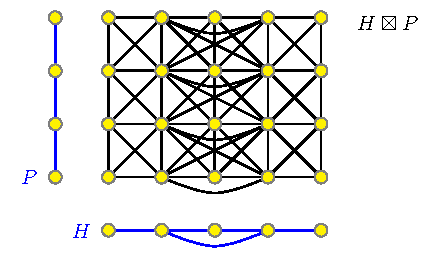
\includegraphics{ProductExample}
\caption{Example of a strong product.}
\label{ProductExample}
\end{figure}

We generalise \cref{PlanarBasic} as follows. 

\begin{thm}
\label{kPlanarBasic}
Every $k$-planar graph is a subgraph of $H\boxtimes P$, for some graph $H$ of treewidth at most $(4+o(1))k^5$ and for some path $P$. 
\end{thm}

This theorem and several related results are proved in \cref{Structure}. In particular, in \cref{sec-1-planar} we present a refinement of \cref{kPlanarBasic} in the case $k=1$. In \cref{sec-g-k-planar} we generalise \cref{kPlanarBasic} for graphs that have a drawing on an arbitrary surface with a bounded number of crossings per edge. 


\cref{kPlanarBasic} (and its generalisations) have applications in diverse areas, including queue layouts  \citep{dujmovic.joret.ea:planar}, non-repetitive colouring  \citep{dujmovic.esperet.ea:planar}, and $p$-centred colouring  \citep{micek:personal}.
%, and graph encoding \citep{BGP}. 
These applications in the context of $k$-planar graphs are explored in \cref{Applications}. For example, we prove that $k$-planar graphs have bounded non-repetitive chromatic number (for fixed $k$). Prior to the recent work of 
\citet{dujmovic.esperet.ea:planar}, it was even open whether planar graphs have bounded non-repetitive chromatic number.

\cref{Characterisation} presents a rough characterisation of $k$-planar graphs in terms of an underlying planar graph. This is useful for showing that various families of graphs are $k$-planar. For example, we conclude that bounded powers of bounded-degree planar graphs are $k$-planar, for a suitable constant $k$. Thus 
\cref{kPlanarBasic} and the above applications are applicable to this class. These results also generalise for arbitrary surfaces. 

\cref{Examples} presents several examples of $k$-planar graphs, including $k$-map graphs, $k$-string graphs, and $k$-nearest neighbour graphs. All of the above results are applicable to these examples. 


%\citet{dujmovic.joret.ea:planar} generalised their result for planar graphs for graphs embeddable on any surface. In particular, they proved that every graph of Euler genus $g$ is a subgraph of $H\boxtimes P$ for some graph $H$ of treewidth at most $???k$ and for some path $P$. We provide a further generalisation allowing crossings. Say a graph is $(g,k)$-planar if it has a drawing in a surface of Euler genus at most $g$ in which each edge is involved in at most $k$ crossings. 
%
%\begin{thm}
%For all integers $g,k\geq 1$ there is an integer $c_{k,g}$, such that every $(g,k)$-planar graph is a subgraph of $H\boxtimes P$, for some graph $H$ of treewidth at most $c_{k,g}$  and for some path $P$. 
%\end{thm}


%In 1965, \citet{ringel:sechsfarbenproblem} introduced the notion of $1$-planar graphs, a generalization of planar graphs that allows edges to cross provided that no edge is involved in more than one crossing. This simple generalization has since become a rich source of problems and results.  Indeed, the annotated bibliography on 1-planar graphs by \cite{kobourov.liotta.ea:annotated} contains more than 140 entries.
%
%The natural generalization of $1$-planar graphs, $k$-planar graphs (that allow edge to be involved in up to $k$ crossings), has been the topic of important recent work on graph drawing. Though planar graphs are, by now, quite well-understood, the situation is much less clear for $k$-planar graphs; even the maximum edge-density of $k$-planar graphs is not completely settled.  For $k\le 4$, the maximum number of edges in an $n$-vertex $k$-planar graph is $(k+3)(n-2)$, which is tight for $k=1,2$ \cite{pach.toth:graphs}.  A near-tight bound of $11(n-2)/2$ is known for $k=3$ \cite{pach.radoicic.ea:improving} but for $k>4$, the current best upper bound is $4.108\sqrt{k}n$ \cite{pach.toth:graphs}.

% In the current paper we investigate the structure of $k$-planar graphs.  Since planarity is closed under taking minors, planar graphs can be characterised by a finite set of forbidden minors.  Indeed, Wagner's Theorem states that this set consists of the complete 5-vertex graph $K_5$ and the complete bipartite graph $K_{3,3}$.  Unfortunately, $k$-planarity is not closed under taking minors, ruling out this kind of clean structural result.  The purpose of the current paper is to extend a new structural result for planar graphs to $k$-planar graphs.

%The purpose of the current paper is to show that new structural results for planar graphs can be extended to $k$-planar graphs.  These results can be used to give a rough characterization of $k$-planar graphs of powers of bounded-degree planar graphs
% Rather, we present a rough structural characterization of $k$-planar graphs that, despite its roughness, provides several new results for $k$-planar and related graph families.  
%All of these results are based on layered $H$-partitions, which we now define.{\color{red}TODO: Help.}


%Thus, like genus-$g$ graphs,$k$-planar graphs are a generalization of planar graphs (which are genus-$0$ graphs).  Unlike genus-$g$ graphs, however, the family of $k$-planar graphs is not minor-closed.  A graph $G'$ obtained from a $k$-planar graph $G$ by edge deletions and edge contractions may or may not be $k$-planar. Indeed, \citet{dujmovic.eppstein.ea:structure} construct 1-planar graphs that contain arbitrarily large complete graph minors.


%\note{PM}{TODO: Write here about applications. non-repetitive colouring, $p$-centered colouring, $(g,k)$-planar graph, $(g,d)$-map graphs, $k$-NN graphs, David's rough characterization.}



%The remainder of the paper is organised as follows: In \cref{k-planar} we prove \cref{sec-k-planar}.  In \cref{sec-1-planar} we prove \cref{1-planar}.   In \cref{g-k-planar} we prove \cref{g-k-planar}. In \cref{consequences} we point out some consequences of these results for some of the other graph parameters mentioned above. \comment{Re-DO}

%%%%%%%%%%%%%%%%%%%%%%%%%%%
\section{Tools}
\label{Tools}

This section defines concepts from from the literature that will be important for our work. 

In this paper, all graphs are finite and undirected. Unless specifically mentioned otherwise, all graphs are also simple. For any graph $G$ and any set $S$ (typically $S\subseteq V(G)$) we use $G[S]$ to denote the graph with vertex set $V(G)\cap S$ and edge set $\{uv\in E(G) : u,v\in S\}$.  We use $G-S$ as a shorthand for $G[V(G)\setminus S]$. We use $G'\subseteq G$ to denote subgraph containment; that is, $V(G')\subseteq V(G)$ and $E(G')\subseteq E(G)$.

We now formally define $k$-planar graphs.  An \emph{embedded graph} $G$ is a graph with $V(G)\subset\R^2$ in which each edge $vw\in E(G)$ is a closed curve\footnote{A closed curve in a surface $\Sigma$ is a continuous function $f:[0,1]\to \Sigma$. The points $f(0)$ and $f(1)$ are called the \emph{endpoints} of the curve.  When there is no danger of misunderstanding we treat a curve $f$ as the point set $\{f(t):0\le t\le 1\}$.} in $\R^2$ with endpoints $v$ and $w$ and not containing any vertex of $G$ in its interior.  A \emph{crossing} in an embedded graph $G$ is a triple $(p,vw,xy)$ with $p\in\R^2$, $vw,xy\in E(G)$ and such that $p\in (vw\cap xy)\setminus\{v,w,x,y\}$. An embedded graph $G$ is \emph{$k$-plane} if each edge of $G$ takes part in at most $k$ crossings.  A (not necessarily embedded) graph $G'$ is \emph{$k$-planar} if there exists $k$-plane graph $G$ isomorphic to $G'$.  Under these definitions, $0$-planar graphs are exactly planar graphs and $0$-plane graphs are exactly plane graphs. 

We now define two concepts used in the statements of \cref{PlanarBasic,kPlanarBasic}: strong products and treewidth. The \emph{strong product} of graphs $A$ and $B$, denoted by $A\boxtimes B$, is the graph with vertex set $V(A)\times V(B)$, where distinct vertices $(v,x),(w,y)\in V(A)\times V(B)$ are adjacent if: 
\begin{compactitem}
\item  $v=w$ and $xy\in E(B)$, or 
\item  $x=y$ and $vw\in E(A)$, or  
\item  $vw\in E(A)$ and $xy\in E(B)$. 
\end{compactitem}
A \emph{tree-decomposition} $\mathcal{K}$ of a graph $G$ consists of a tree $K$ and a collection $\mathcal{K}=(B_x:x\in V(K))$ of subsets of $V(G)$ indexed by the nodes of $K$ such that:
\begin{compactenum}[(i)]
\item for every $vw\in E(G)$, there exists some $x\in V(K)$ with $v,w\in B_x$; and 
\item for every $v\in V(G)$, the induced subgraph $K[x] := K[\{y: x\in B_y\}]$ is connected.  
\end{compactenum}
The \emph{width} of the tree-decomposition $\mathcal{K}$ is $\max\{|B_x|:x\in V(K)\}-1$.  The \emph{treewidth} $\tw(G)$ of a graph $G$ is the minimum width of a tree-decomposition of $G$.  Treewidth is the standard measure of how similar a graph is to a tree. Indeed, a connected graph has treewidth 1 if and only if it is a tree. Treewidth is of fundamental importance in structural and algorithmic graph theory; see \citep{Reed03,HW17,Bodlaender-TCS98} for surveys. 

While strong products enable an easy statement of \cref{PlanarBasic,kPlanarBasic}, to prove such theorems it is helpful to work with layerings and partitions, which we now introduce. A \emph{layering} of a graph $G$ is a sequence $\mathcal{L}=\langle V_0,V_1,\ldots\rangle$ such that $\{V_0,V_1,\ldots\}$ is a partition of $V(G)$ and for every edge $vw\in E(G)$, if $v\in V_i$ and $w\in V_j$ then $|j-i|\leq 1$.  For any partition $\mathcal{P}=\{S_1,\ldots,S_p\}$ of $V(G)$, a \emph{quotient graph} $H=G/\mathcal{P}$ has a $p$-element vertex set $V(H)=\{x_1,\ldots,x_p\}$ and $x_ix_j\in E(H)$ if and only if there exists an edge $vw\in E(G)$ such that $v\in S_i$ and $w\in S_j$. To highlight the importance of the quotient graph $H$, we call $\mathcal{P}$ an \emph{$H$-partition} and write this concisely as $\mathcal{P}=\{S_x : x\in V(H)\}$ so that each element of $\mathcal{P}$ is indexed by the vertex it creates in $H$.\footnote{An alternative definition of a layering of $G$ is an $H$-partition of $G$ where $H$ is a path.}  A layered $H$-partition $(\mathcal{L},\mathcal{P})$ of a graph $G$ consists of a layering $\mathcal{L}$ of $G$ and an $H$-partition $\mathcal{P}$ of $G$. The \emph{layered width} of $(\mathcal{L},\mathcal{P})$ is $\max\{|L\cap P|: L\in\mathcal{L},\, P\in\mathcal{P}\}$. These definitions relate to strong products as follows. 

\begin{lem}[\citep{dujmovic.joret.ea:planar}] 
\label{PartitionProduct}
For every graph $H$, a graph $G$ has an $H$-partition of layered width at most $\ell$ if and only if $G$ is a subgraph of 
$H \boxtimes P \boxtimes K_\ell$ for some path $P$.
\end{lem}

\citet{dujmovic.joret.ea:planar} also showed it suffices to consider partitions of layered width 1.

\begin{lem}[\citep{dujmovic.joret.ea:planar}] 
\label{MakeWidth1}
If a graph $G$ has an $H$-partition of layered width $\ell$ with respect to layering $\langle V_0,V_1,\dots\rangle$, for some graph $H$ of treewidth at most $k$, then $G$ has an $H'$-partition of layered width 1 with respect to the same layering, for some graph $H'$ of treewidth at most $(k+1)\ell-1$.  That is, if $G\subseteq H\boxtimes P\boxtimes K_\ell$ for some graph $H$ of treewidth at most $k$  and for some path $P$, then $G\subseteq H' \boxtimes P$ for some graph $H'$ of treewidth at most $(k+1)\ell-1$.
\end{lem}

\citet{dujmovic.joret.ea:planar} proved the following result, which with \cref{PartitionProduct,MakeWidth1}, implies \cref{PlanarBasic}. 

\begin{thm}[\citep{dujmovic.joret.ea:planar}]
\label{PlanarPartition}
Every planar graph has:
\begin{compactitem}
\item an $H$-partition of layered width $1$ for some planar graph $H$ of treewidth at most $8$, and
\item an $H$-partition of layered width $3$ for some planar graph $H$ of treewidth at most $3$.
\end{compactitem}
\end{thm}

%Layered $H$-partitions of small layered width in which $H$ has some additional property are a useful tool for a number of graph problems.  One such useful property is small \emph{treewidth}, which we now define. 

% \citet{dujmovic.joret.ea:planar} show that, if each graph $G$ in some family $\mathcal{G}$ of graphs has a layered $H$-partition for which the layered width of the partition and the treewidth of $H$ are each upper-bounded by some constant $c_\mathcal{G}$, then each of the following quantities are upper bounded by a constant, for every $G\in\mathcal{G}$: queue number, track number, and layered treewidth. \citet{dujmovic.esperet.ea:planar} add non-repetitive chromatic number to this list.  \citet{dujmovic.joret.ea:planar} show that two common families of graphs have such $H$-partitions: planar graphs, graphs of bounded genus, and (more generally) apex-minor-free graphs.

% In this paper we show that another family of graphs admits layered $H$-partitions of bounded layered width in which $H$ has bounded treewidth:

\citet{dujmovic.joret.ea:planar} proved the following generalisation of \cref{PlanarBasic,PlanarPartition} for graphs embeddable on other surfaces.\footnote{The \textit{Euler genus} of the orientable surface with $h$ handles is $2h$. The \textit{Euler genus} of the non-orientable surface with $c$ cross-caps is $c$. The \textit{Euler genus} of a graph $G$ is the minimum integer $g$ such that $G$ embeds in a surface of Euler genus $g$. Of course, a graph is planar if and only if it has Euler genus 0; see \citep{mohar.thomassen:graphs} for more about graph embeddings in surfaces.}

\begin{thm}[\citep{dujmovic.joret.ea:planar}]
\label{SurfacePartition}
Every graph of Euler genus $g$ is a subgraph of:
\begin{compactenum}[(a)]
\item  $H \boxtimes P \boxtimes K_{\max\{2g,1\}}$ for some graph $H$ of treewidth at most $9$ and for some path $P$;
\item  $H \boxtimes P \boxtimes K_{\max\{2g,3\}}$ for some graph $H$ of treewidth at most $4$ and for some path $P$;
\item $(K_{2g} + H )  \boxtimes P$ for some graph $H$ of treewidth at most $8$  and some path $P$. 
\end{compactenum}
Equivalently, every graph of Euler genus $g$ has:
\begin{compactenum}[(a)]
\item an $H$-partition with layered width at most $\max\{2g,1\}$ such that $H$ has treewidth at most $9$;
\item an $H$-partition with layered width at most $\max\{2g,3\}$ such that $H$ has treewidth at most $4$; 
\item an $H$-partition with layered width at most $1$ such that $H$ has treewidth at most $2g+7$. 
\end{compactenum}
%\textcolor{red}{eliminate some of these results?}
\end{thm}

\citet{dujmovic.joret.ea:planar} generalised \cref{SurfacePartition} further to show that for every apex\footnote{A graph $M$ is a \textit{minor} of a graph $G$ if a graph isomorphic to $M$ can be obtained from a subgraph of $G$ by contracting edges. A class $\mathcal{G}$ of graphs is \emph{minor-closed} if for every graph $G\in\mathcal{G}$, every minor of $G$ is in $\mathcal{G}$. A minor-closed class is \emph{proper} if it is not the class of all graphs. For example, for fixed $g\geq 0$, the class of graphs with Euler genus at most $g$ is a proper minor-closed class. A graph $G$ is $t$-apex if it contains a set $A$ of at most $t$ vertices such that $G-A$ is planar. A 1-apex graph is \emph{apex}.  A minor-closed class $\mathcal{G}$ is apex-minor-free if some apex graph is not in $\mathcal{G}$.}
 graph $X$, there is a constant $c$ such that every $X$-minor-free graph is a subgraph of $H\boxtimes P$ for some graph $H$ of treewidth at most $c$. Apex-minor-free graphs are the largest minor-closed class for which such a theorem holds \citep{dujmovic.joret.ea:planar}. However, the family of $k$-planar graphs is not minor-closed.  A graph $G'$ obtained from a $k$-planar graph $G$ by edge deletions and edge contractions may or may not be $k$-planar. Indeed, \citet{dujmovic.eppstein.ea:structure} construct 1-planar graphs that contain arbitrarily large complete graph minors. Our results for $k$-planar graphs are the first of this type for a non-minor-closed class. 

The following is the main result of this paper; it shows that $k$-planar graphs admit $H$-partitions with bounded layered width, in which $H$ has bounded treewidth. With \cref{PartitionProduct,MakeWidth1}, this proves \cref{kPlanarBasic}. % with $c_k\leq(4+o(1))k^5$.

\begin{thm}
\label{k-planar}
Every $k$-planar graph has a layered $H$-partition of layered width at most $24k^2 + 60k + 36$ in which $H$ has treewidth at most $\treewidth$.
\end{thm}

 
In the special case $k=1$ we obtain better constants and an additional property (planarity) of $H$:

\begin{thm}
\label{1-planar}
Every 1-planar graph has a layered $H$-partition of layered width at most 30 where $H$ is planar and has treewidth at most 3.
\end{thm}

%These results imply that $k$-planar graphs have all the graph parameters mentioned above upper-bounded by some constant $c_k$.

Prior to this work, the strongest structural description of $k$-planar graphs was in terms of layered treewidth, which we now define.  A \emph{layered tree-decomposition} $(\mathcal{L},\mathcal{K})$ consists of a layering $\mathcal{L}$ and a tree-decomposition $\mathcal{K}$ of $G$. The layered width of $(\mathcal{L},\mathcal{K})$ is $\max\{|L\cap B|: L\in \mathcal{L},\, B\in \mathcal{K}\}$.  The \emph{layered treewidth} of $G$ is the minimum layered width of any layered tree-decomposition of $G$. \citet{dujmovic.morin.ea:layered} proved that planar graphs have layered treewidth at most 3, that graphs of Euler genus $g$ have layered treewidth at most $2g+3$, and more generally that a minor-closed class has bounded layered treewidth if and only if it excludes some apex graph. \citet{dujmovic.eppstein.ea:structure} show that $k$-planar graphs have layered treewidth at most $6(k+1)$.  

If a graph has a partition with bounded layered width, where the quotient has bounded treewidth, then the graph has bounded layered treewidth. In particular, suppose that an $n$-vertex graph $G$ has an $H$-partition with layered width at most $\ell$ such that $H$ has treewidth at most $k$. \citet{dujmovic.joret.ea:planar} proved that $G$ has layered treewidth at most $(k+1)\ell$. So any property that holds for graphs of bounded layered treewidth also holds for $G$. For example, Norin proved that every $n$-vertex graph with layered treewidth at most $t$ has treewidth less than $2\sqrt{tn}$ (see \citep{dujmovic.morin.ea:layered}). Thus, $G$ has treewidth at most $2\sqrt{(k+1)\ell n}$. This in turn leads to a $O(\sqrt{(k+1)\ell n})$ balanced separator theorem for such graphs \citep{RS-II}. So, in the case of $k$-planar graphs, \cref{k-planar} implies an analogue of the separator theorem of \citet{FP08} mentioned in the introduction, albeit with worse dependence on $k$. What sets layered partitions apart from layered treewidth is that they lead to constant upper bounds on the queue-number  and non-repetitive chromatic number, whereas for both these parameters, the best known upper bound obtainable via layered treewidth is $O(\log n)$; see \cref{Applications}. 

%Indeed the former structure leads to $O(1)$ bounds on the queue-number, instead of $O(\log n)$ bounds obtained via layered treewidth. That said, it is open whether graphs of bounded layered treewidth have bounded queue-number. It is even possible that graphs of bounded layered treewidth have partitions of bounded layered width, whose quotient has bounded treewidth.
%
%This already implies that several of the graph parameters mentioned above, including queue-number and non-repetitive chromatic number are upper-bounded by $O(k\log n)$ for $n$-vertex $k$-planar graphs \cite{dujmovic.morin.ea:layered}. \cref{k-planar} is a significant strengthening of this result. It implies that $k$-planar graphs have layered treewidth bounded by a function of $k$, and gives upper bounds on the queue-number and non-repetitive chromatic number of $n$-vertex $k$-planar graphs that are independent of $n$.
%


%%%%%%%%%%%%%%%%%%%%%%%%%%%
\section{Structure}
\label{Structure}

The purpose of this section is to prove \cref{k-planar} and related structural results. 
We begin by introducing a tool for studying planar graphs, called a tripod decomposition, that is implicit in previous work on $H$-partitions of planar graphs \cite{dujmovic.joret.ea:planar}.  We then show how the tripod decomposition of a planarised version of a $k$-planar graph $G$ can be used to find a layered $H$-partition of $G$ of small layered width in which $H$ has small treewidth. 

\subsection{Tripod Decompositions}
\label{TripodDecompositions}

Let $T$ be a tree rooted at some node $r\in V(T)$. The \emph{$T$-depth} of a node $x\in V(T)$ is equal to the length of the path from $x$ to $r$ in $T$. A path $P$ in $T$ is \emph{vertical} if, for each integer $i$, $P$ contains at most one vertex of $T$-depth $i$.  The deepest vertex in a vertical path $P$ is called  the \emph{lower endpoint} of $P$ and the shallowest vertex in $P$ is called the \emph{upper endpoint} of $P$. For each node $v\in V(T)$, we call each node on the path, in $T$, from $v$ to $r$ (including $v$ itself) a \emph{$T$-ancestor} of $v$.  If $v'$ is a $T$-ancestor of $v$, then $v$ is a \emph{$T$-descendant} of $v'$.

A \emph{near-triangulation} $N$ is a plane graph whose outer face, $F$, is bounded by a simple cycle in $N$ and each of whose inner faces is bounded by a 3-cycle in $N$.  A \emph{triangulation} is a near-triangulation whose outer face is bounded by a 3-cycle.  For any cycle $F$ in a near-triangulation $N$ we use $N\llparenthesis F\rrparenthesis$ to denote the near-triangulation consisting of all the edges and vertices of $N$ that are contained in $F$ or its interior.

For a connected graph $G$ and two vertices $v,w\in V(G)$, we use $\dist_{G}(v,w)$ to denote the length of a shortest path, in $G$, with endpoints $v$ and $w$.  For a vertex $r\in V(G)$, the \emph{BFS layering} of $G$ from $r$ is the layering $\langle V_0,V_1,\ldots\rangle$ of $G$ where $V_i=\{v\in V(G): \dist_{G}(r,v)=i\}$ for each integer $i\ge 0$.  A \emph{BFS spanning tree} $T$ of $G$ rooted at $r$ is a spanning tree of $G$ rooted at $r$ where, for every $v\in V(G)$, $\dist_T(v,r)=\dist_G(v,r)$.

For the remainder of this section, $\Delta$ is a triangulation, $r$ is a degree-3 vertex on the outer face of $\Delta$, and $T$ is a BFS spanning tree of $\Delta$ rooted at $r$.

Fix some cycle $F$ in $\Delta$ and let $N=\Delta\llparenthesis F\rrparenthesis$.
Let $\tau=v_1v_2v_3$ be an inner face of $N$ and consider the three minimal vertical paths $Q_1$, $Q_2$, and $Q_3$ in $T$ such that, for each $i\in\{1,2,3\}$ the lower endpoint of $Q_i$ is $v_i$ and the upper endpoint $v_i'$ of $Q_i$ is in $V(F)$.  If $Q_1$, $Q_2$, and $Q_3$ are vertex-disjoint, then the graph $\overline{Y}:=\tau\cup Q_1\cup Q_2\cup Q_3$ is called the \emph{closed tripod} in $N$ determined by $\tau$.  We call $Q_1$, $Q_2$, and $Q_3$ the \emph{legs}, $v_1'$, $v_2'$ and $v_3'$ the \emph{feet}, and $\tau$ the \emph{crotch} of $\overline{Y}$.  We call $Y:=\overline{Y}-F$ the \emph{(open) tripod} of $N$ determined by $\tau$.  The graph $M:=\overline{Y}\cup F$ is called a \emph{Mercedes graph} and the (at most three) inner faces of $M$ other than $\tau$ are called the \emph{wedges} of $M$.

Let $r$ be a degree-3 node on the outer face of a triangulation $\Delta$.  A \emph{tripod decomposition}  $K=K(\Delta, T, r)$ is a rooted tree in which each non-root node $x\in V(K)$ is associated with several objects (refer to \cref{K-node}):

\begin{figure}
  \begin{center}
    \begin{tabular}{cc}
      \includegraphics{figs/K-node-1} &
      \includegraphics{figs/K-node-2}
    \end{tabular}
  \end{center}
  \caption{The elements associated with a node $x\in V(K)$.}
  \label{K-node}
\end{figure}

\begin{enumerate}
  \item A cycle $F_x$ in $\Delta$ and the near-triangulation $N_x:=\Delta\llparenthesis F_x\rrparenthesis$.
  
  \item An inner face $\tau_x$ of $N_x$ that determines a closed tripod $\overline{Y}_x$ and an open tripod $Y_x:=\overline{Y}_x-F_x$ in $N_x$, both with crotch $\tau_x$.
  
  \item The \emph{Mercedes graph} $M_x:=F_x\cup \overline{Y}_x$
\end{enumerate}

The root node $r^0_K$ of $K$ is exceptional.  We define $F_{r^0_K}$ to be the single-vertex graph containing $r$, we define $\overline{Y}_{r^0_K}$ to be the star formed by $r$ and its three neighbours in $\Delta$, and (as usual) $Y_{r^0_K}:=\overline{Y}_{r^0_K}-F_{r^0_K}$.  The root node $r^0_K$ has exactly one child $r_K$, called the \emph{sub-root} of $K$, for which $F_{r_K}$ is the 3-cycle formed by the neighbours of $r$ in $\Delta$.

The non-root nodes of the tripod decomposition $K$ (including the sub-root $r_K$) satisfy the following conditions:
\begin{enumerate}[(PR1)]
  \item \PRlabel{children} For each non-root node $x\in V(K)$ such that $M_x$ has $f\le 3$ wedges $F_{x,1},\ldots,F_{x,f}$, the node $x$ has exactly $f$ children $y_1,\ldots,y_f$ in $K$ and $F_{y_i} = F_{x,i}$ for each $i\in\{1,\ldots,f\}$.
  
  \item \PRlabel{ancestor-boundary} For each non-root node $x\in V(K)$, there exists a partition of $V(F_x)$ into $g\le 3$ non-empty sets $P_1,\ldots,P_g$ such that, for each $i\in\{1,\ldots,g\}$, $F[P_i]$ is a path that is contained in $Y_a$ for some $K$-ancestor $a$ of $x$. 
  
  \item \PRlabel{tripod-feet} For each $i\in\{1,\ldots,g\}$, at least one vertex in $P_i$ is a foot of the closed tripod $\overline{Y}_x$.

  \item \PRlabel{partition} $\{Y_x : x\in V(K)\}$ is a partition of $V(\Delta)\setminus\{r\}$.
\end{enumerate}

For any triangulation $\Delta$ in which the outer face has a vertex $r$ of degree 3 and for any BFS spanning tree of $\Delta$ rooted at $r$, there exists a tripod decomposition $K=K(\Delta,T,r)$.  Indeed, this tree is constructed (albeit implicitly) by \citet[Proof of Lemma~14]{dujmovic.joret.ea:planar}.\footnote{\citet{dujmovic.joret.ea:planar} do not require that $T$ be a BFS spanning tree, only that its root, $r$ has degree 3 in $\Delta$ and in $T$.}


% The following claim is not used until later in the paper. However, it's proof is a helpful exercise in understanding the properties of a PS-Tree.
% 
% \begin{clm}\label{strong-ancestor-boundary}
%   Let $K$ be a PS-tree and
%   let $y\in V(K)$ be a non-root node with parent $p$ such that $V(F_y\cap Y_a)\neq\emptyset$ for some $K$-ancestor $a\neq p$ of $p$. Then $V(F_p\cap Y_a)\neq\emptyset$.
% \end{clm}
% 
% \begin{proof}
%   By \propref{children}, $F_y$ is a wedge in the Mercedes graph $M_p$, so $V(F_y)$ can be partitioned into  $P_1'=V(F_y\cap Y_p)$ and $P_{2,3}'=V(F_y\cap F_p)$.  Let $P_1,\ldots,P_g$ denote the partition of $V(F_p)$ given by \propref{ancestor-boundary}.  
% 
%   We claim that \PRref{tripod-feet} ensures that $P_{2,3}'\subset P_i\cup P_j$ for some $i,j\in \{1,\ldots,g\}$.  If $g=2$, this claim is immediate, so assume $g=3$. Then, $F_y\cap \overline{Y}_p$ is the path formed by two legs $Q_2$ and $Q_3$ of $\overline{Y}_p$ and one edge $v_2v_3$ of $\tau_p$.  
%   By \PRref{tripod-feet} and the assumption that $q=3$, $Q_2$ has a foot $v_2'\in P_i$ and $Q_3$ has a foot $v_3'\in P_j$, for some $i\neq j$.  The third foot $v_1'$ of $\overline{Y}_p$ is therefore in $P_\ell$ for the unique $\ell \in\{1,2,3\}\setminus \{i,j\}$.  It follows that $V(P_\ell\cap F_y)=\emptyset$.
% 
%   Setting $P_2'=V(P_i\cup F_y)$ and $P_3'=V(P_j\cup F_y)$ yields a partition $\{P_1',P_2',P_3'\}$ of $V(F_y)$ such that $P_1'\subset V(Y_{p})$,   
%   $P_2'\subset V(Y_{a_2})$, and $P_3'\subset V(Y_{a_3})$  for some $K$-ancestors $a_2$ and $a_3$ of $a$.  Therefore $a_2$ and $a_3$ are the only $K$-ancestors $a\neq p$ of $p$, such that $V(F_y\cap Y_a)\neq\emptyset$.
%   Now, each foot $v_2',v_3'\in V(F_p)$.  Furthermore, $v_2'\in P_i\subseteq V(Y_{a_2})$ and $v_3'\in P_j\subseteq V(Y_{a_3})$. Therefore, $V(F_p\cap Y_{a_2})\supseteq\{v_2'\}\neq\emptyset$ and $V(F_p\cap Y_{a_3})\supseteq\{v_3'\}\neq\emptyset$, as claimed.
% \end{proof}
% 
% Contained in the proof of \clmref{strong-ancestor-boundary} is the following addendum to \propref{ancestor-boundary}:
% 
% \begin{enumerate}[(PR1')]\setcounter{enumi}{1}
%   \item \proplabel{ancestor-boundary-ii} Furthermore, if $g=3$, then  $P_i=V(F_x\cap Y_p)$ where $p$ is the parent of $x$ in $K$, for one $i\in\{1,2,3\}$.
% \end{enumerate}

% \subsubsection{Layered $H$-Partitions from PS-Trees}
% \seclabel{k-to-h}
% 
% Before continuing, it is worth pointing out how an $H$-partition of $\Delta-\{r\}$ can be obtained from a PS-tree $K=K(\Delta,T,r)$. (Note: There is nothing new in this section.  This is just an alternative presentation of material from \citet{dujmovic.joret.ea:planar}.) Given $K=K(\Delta,T,r)$, we obtain a layered $H$-partition $(\mathcal{L},\mathcal{P})$ as follows. 
% 
% We use the layering $\mathcal{L}=\{V_0,V_1,\ldots,V_h\}$ where $V_i=\{ v\in V(\Delta)\setminus\{r\}: \dist_{\Delta}(r,v)=i\}$ and $h=\max\{\dist_\Delta(r,v):v\in V(\Delta)\}$.  The fact that $T$ is a BFS tree ensures that $\mathcal{L}$ is, indeed, a layering of $\Delta-\{r\}$.  We use the vertex partition $\mathcal{P}=\{ S_x:=V(Y_x) : x\in V(K)\}$.  \PRref{partition} ensures that $\mathcal{P}$ is, indeed a partition of $V(\Delta)-\{r\}$.
% 
% The resulting layered $H$-partition $(\mathcal{L},\mathcal{P})$ has layered width at most 3 because, for each $x\in V(K)$, $S_x$ is made up of vertices from at most 3 vertical paths in $T$.  These are either the three vertices of $Y_{r_k}$ (if $x=r_K$) or the vertices of the open tripod $Y_x$ whose vertices are included in three vertical paths $Q_1,Q_2,Q_3$ that form the legs of the closed tripod $\overline{Y}_x$.  Therefore $|S_x\cap V_i|\le 3$.
% 
% To show that the quotient graph $H=\Delta/\mathcal{P}$ has small treewidth, we produce a tree-decomposition $\mathcal{K}=\{B_x: x\in V(K)\}$ of $H$ using the tree $K$.  For each $x\in V(K)$, the subtree $K[x]=K[\{y:x\in B_y\}]$ contains
% $x$ as well as every node $y$ such that $V(Y_x)\cap V(F_y) \neq\emptyset$.
% It is straightforward to verify that $K[x]$ is connected for each $x\in V(K)$. The fact that $F_x$ is a cycle in $\Delta$ and \propref{ancestor-boundary} ensures that, if $xy\in E(H)$, then one of $x$ or $y$ is a $K$-ancestor of the other. \propref{ancestor-boundary} also implies that, for any node $y\in V(K)$, $|B_y|\le 4$, since $B_y$ contains $y$ and at most 3 $K$-ancestors of $y$.
% 
% Therefore $(\mathcal{L},\mathcal{P})$ is a layered $H$-partition of $\Delta-\{r\}$ with layered width 3 in which $H$ has treewidth 3.  Furthermore, for each $P\in\mathcal{P}$, $\Delta[P]$ is connected.  Since $\Delta$ is planar, this implies that $H$ is planar.\footnote{It is well-known and easy to see that any graph $\Delta'$ obtained by contracting an edge in a planar graph $\Delta$ is also planar.  Repeatedly applying this fact implies that $\Delta/\mathcal{P}$ is planar provided that $\Delta[P]$ is connected for every $P\in\mathcal{P}$.}

\subsection{$k$-Planar Graphs}
\label{sec-k-planar}

Let $G$ be a $k$-plane graph.  We will assume, for ease of exposition, that any point $p\in\R^2$ is involved in at most one crossing $(p,vw,xy)$ of $G$. This assumption is not critical since it can be enforced by a slight deformation of the edges of $G$ and the resulting (deformed) graph is also $k$-plane.   Consider the following plane graphs (see \cref{wrapper}(a)):
\begin{compactenum}
  \item Add a dummy vertex at each crossing in $G$ to obtain a plane graph and then add edges to this graph to obtain a triangulation $G^+$.
  
  \item Add a complete graph $K_4$ that contains $G^{+}$ in one of its inner faces, $F_0$, and then add edges to the resulting graph to obtain a triangulation $G^{++}$.
\end{compactenum}
Observe that, for any edge $vw\in E(G)$, 
\begin{equation}  
  \dist_{G^+}(v,w) \le k+1 \enspace ,  \eqlabel{distance-preserving}
\end{equation}
since (the curve) $vw$ contains a sequence $W_{vw}$ of at most $k+2$ vertices of $G^+$ that form a walk from $v$ to $w$ in $G^+$.

\begin{figure}
  \begin{center}
    \begin{tabular}{c@{\hspace{2cm}}c}
      \includegraphics{figs/wrapper-1} &
      %\includegraphics{figs/wrapper-3} &
      \includegraphics{figs/wrapper-3} \\
      (a) & (b) 
    \end{tabular}
  \end{center}  
  \caption{Wrapping a $K_4$ around $G^+$: (a)~the graph $G^{++}$
  %, (b)~the spanning tree $T$ of $G^{++}$, 
  and (b)~the modified version of $G^{++}$ used in the proof of \cref{cor-k-planar}.}
  \label{wrapper}
\end{figure}

Let $r$ be the vertex of the $K_4$ not incident on $F_0$ and let $T$ be a BFS spanning tree of $G^{++}$ rooted at $r$. 
For each integer $i\ge 0$, let $V_i:=\{v\in V(G^+): \dist_{T}(r,v)=i\}$ and observe that $\{V_2,V_3,\ldots,V_{h}\}$ is a layering of $G^+$ (but not of $G$).

Let $K=K(G^{++},T,r)$ be a tripod decomposition and observe that the sub-root $r_K$ of $K$ has $F_{r_K}=F_0$.  This implies:
\begin{compactenum}[(PR1)]\setcounter{enumi}{4}
  \item \PRlabel{all-in}  $G^+\subseteq N_{r_K}-F_{r_K}$.
\end{compactenum}

For each vertex $z\in V(G^+)$, let $P_z=\{a\in V(K): z\in V(N_a-F_a)\}$.  By \PRref{all-in}, $P_{z}$ contains the sub-root $r_K$ of $K$.  By \PRref{children}, any node $x\in P_z$ has at most one of its children in $P_z$ and any node $x'\not\in P_z$ has none of its children in $P_z$.  Therefore $K[P_z]$ is a vertical path in $K$ that contains $r_K$ (and whose lower endpoint is the unique node $x\in V(K)$ such that $z\in Y_x$). We are about to repeatedly use the fact that the common intersection of two or more vertical paths is a vertical path. 

For each edge $vw\in E(G)$, consider the walk $W_{vw}$ in $G^+$ that corresponds to the sequence of vertices in $G^+$ encountered while walking along the curve $vw$ from $v$ to $w$. We define $A_{vw}:=\bigcap_{z\in W_{vw}} P_z$.  Since $V(W_{vw})\subseteq V(G^+)$, $A_{vw}$ is well-defined.  For each $z\in V(W_{vw})$, $K[P_{z}]$ is a vertical path in $K$ that contains $r_K$.   Therefore $K[A_{vw}]$ is a vertical path in $K$ that contains $r_K$.  For each vertex $v\in V(G)$ define $A_v:=\bigcap_{vw\in E(G)} A_{vw}$.  Again, $K[A_v]$ is a vertical path in $K$ that contains $r_K$.  We define $a(v)$ to be the lower endpoint of $K[A_v]$.  In words, $a(v)$ is the lowest node in $K$ such that the interior of $F_{a(v)}$ contains all the edges of $G$ incident to $v$.

For each node $x\in V(K)$, define the \emph{separator}
\[
   S_x := \{v\in V(G): a(v)=x \} \enspace .
\]
Clearly $\mathcal{S}:=\{S_x:x\in V(K)\}$ is a partition of $V(G)$.  We will use $\mathcal{S}$ as the partition that defines our quotient graph $H:=G/\mathcal{S}$ with vertex set $V(H):=V(K)$ and the edge $xy\in E(H)$ if and only if there exists an edge $vw\in E(G)$ with $v\in S_x$ and $w\in S_y$.  First we argue that this partition has small layered width with respect to the layering $\{V_2,V_3,\ldots\}$ of $G^+$ defined by $T$.
 % (recall that this is a layering of $G^+$, not a layering of $G$).

\begin{clm}\label{chargeback-to-y}
   For any $x\in V(K)$ and any vertex $v\in S_x$, there exists an edge $vw\in E(G)$ and a vertex $v'\in Y_x\cap V(W_{vw})$ such that $|\dist_T(r,v')-\dist_T(r,v)|\le k+1$.
\end{clm}

\begin{proof}
  Since $v\in S_x$, the lower endpoint of $K[A_{vw}]$ is $x$ for some edge $vw\in E(G)$.  This implies that $W_{vw}\subseteq N_x-F_x$ but $W_{vw} \not\subseteq N_{x'}-F_{x'}$ for every child $x'$ of $x$ in $K$. Therefore, \PRref{children} and \PRref{ancestor-boundary} imply that $W_{vw}$ contains a vertex $v'\in Y_x$.  Since $G$ is $k$-planar, the length of $W_{vw}$ is at most $k+1$.  Therefore, $\dist_{G^{++}}(v,v') \le k+1$.
  By the triangle inequality,     
  \[
    \dist_{G^{++}}(r,v') \le \dist_{G^{++}}(r,v) + \dist_{G^{++}}(v,v') 
       \le \dist_{G^{++}}(r,v) + k + 1 \enspace .
  \]
  Similarly, $\dist_{G^{++}}(r,v) \le \dist_{G^{++}}(r, v') + k+1$.  Therefore
  $|\dist_{G^{++}}(r,v)-\dist_{G^{++}}(r,v')| \le k+1$ which establishes the claim, since $T$ is BFS spanning tree of $G^{++}$ rooted at $r$, so $\dist_{T}(r,z)=\dist_{G^{++}}(r,z)$ for all $z\in V(G^+)$.
\end{proof}

\begin{clm}
\label{width-of-g-plus}
  For any $x\in V(H)$, and any integer $i\ge 0$, $|S_x\cap V_i|\le 24k+36$.
\end{clm}

\begin{proof}
  Since the vertices of $Y_x$ come from at most three vertical paths in $T$, $|V(Y_x)\cap V_i|\le 3$.  \cref{chargeback-to-y} shows that, for any $v\in S_x\cap V_i$, there exists $vw\in E(G)$ and $v'\in Y_x\cap V(W_{vw})$ with $\dist_T(v,v')\le k+1$. Therefore, $v'\in V(Y_x)\cap V_{j}$ for some $j\in\{i-k-1,\ldots,i+k+1\}$.  If $v'=v$ (so $v'\in V_i$) then $v'$ contributes only one vertex to $S_x$.  If $v'\neq v$ then $v'\in V(G^+)\setminus V(G)$ is a point where two edges of $G$ cross and $v'$ contributes at most the four endpoints of these edges to $S_x$. In either case, each $v'\in V(Y_x)\cap \bigcup_{j=i-k-1}^{i+k+1} V_j$ contributes at most four vertices to $S_x\cap V_i$, so $|S_x\cap V_i|\le 3\times 4\times (2k+3) = 24k+36$.
\end{proof}

Next we describe a tree decomposition $(B_x:x\in V(K))$ of $H$.  We deliberately use the same node set $V(H)=V(K)$ here, because the subtree $K[x]:=K[\{z:x\in B_z\}]$ will be rooted at $x$.  

\begin{clm}\label{xy-ancestor}
   For every edge $xy\in V(H)$, one of $x$ or $y$ is a $K$-ancestor of the other.
 \end{clm}
 
 \begin{proof}
   Since $xy\in E(H)$, there exists an edge $vw\in E(G)$ such that $v\in S_x$ and $w\in S_y$.  By definition, $x\in A_v\subseteq A_{vw}$ and $y\in A_w\subseteq A_{vw}$.  Since $K[A_{vw}]$ is a vertical path in $K$, it follows that one of $x$ or $y$ is a $K$-ancestor of the other. 
\end{proof}

The tree decomposition $(B_x:x\in V(K))$ of $H$ is defined as follows: For each edge $xy\in E(H)$ where $y$ is a $K$-ancestor of $x$, we add $y$ to $B_{x'}$ for every node $x'$ on the path from $x$ to $y$ in $K$.  That this produces a tree-decomposition is due to \cref{xy-ancestor}.  What remains is to upper bound the width of this decomposition.

\begin{clm}\label{bag-size}
  The tree decomposition $(B_x: x\in V(K))$ of $H$ contains no bag larger than $\bagsize$.
\end{clm}

\begin{proof}
  Fix some node $x\in V(K)$ and consider the contents of $B_x$.  By \cref{xy-ancestor}, $B_x$ contains only $K$-ancestors of $x$ (including $x$ itself). 
  
  Consider the graph $A$ that contains the edges and vertices of $F_{a}$ for all $K$-ancestors $a$ of $x$. See \cref{A}(a).  It is helpful to think of this graph as follows:  We begin with $F_{a_0}$ where $a_0:=r_K$ is the root of $K$.  We then cut $F_{a_0}$ into two pieces $F^{\bar{x}}_{a_0}$ and $F^x_{a_0}$ where $F^x_{a_0}$ is the piece that contains $F_x$. (The path that makes this cut contains two legs $Q_i$ and $Q_j$ of a tripod $Y$ and one edge $v_iv_j$ of its crotch $\tau=v_1v_2v_3$.)  This process continues by partitioning $F_{a_1}:=F^x_{a_0}$ recursively.  The process terminates after some number $d$ of iterations, when $F^x_{a_{d-1}}=F_x=F_{a_d}$.

  \begin{figure}
    \begin{center}
      \begin{tabular}{cc}
        \includegraphics{figs/A-1} &
        \includegraphics{figs/A-3} \\ (a) & (b)
      \end{tabular}
    \end{center}
    \caption{(a)~the graph $A$ and (b)~the walks $W_{vw}$ and $W_{ww'}$ that contain the walk $w=v_0,v_1\ldots,v_{\ell-1},v_\ell=w^*$.}
    \label{A}
  \end{figure}

  Refer to \cref{A}(b).  If $B_x$ contains some $K$-ancestor $a_\delta$, $\delta\in\{0,\ldots,d-1\}$, of $x$, it is because there is an edge $vw\in E(G)$ with $w\in S_{a_\delta}$ and $v\in S_{x'}$ for some $K$-descendant $x'$ of $x$.  The edge $vw$ corresponds to a walk $W_{vw}$ in $G^+$. The walk $W_{vw}$ is contained in $N_x-F_x$, otherwise $x\not\in A_{vw}$ which would imply that $x'\not\in A_{vw}$, $x'\not\in A_v$, and $a(v)\neq x'$, contradicting the fact that $v\in S_{x'}$.
  
  However, $w\in S_{a_\delta}$, so there exists an edge $ww'\in E(G)$ such that $W_{ww'}\subseteq N_{a_\delta}-F_{a_\delta}$ but $W_{ww'}\not\subseteq N_{a_{\delta+1}}-F_{a_{\delta+1}}$.  Therefore $W_{ww'}$ must contain a first vertex $w^*\in V(F_{a_{\delta+1}}-F_{a_\delta})\subseteq Y_{a_\delta}$.

  Summarizing, we have a walk $w=v_0,v_1\ldots,v_{\ell-1},v_\ell=w^*$ in $G^+$ such that
  \begin{compactenum}[(i)]
    \item $v_0\in V(N_x-F_x)$;
    
    \item $v_0,\ldots,v_{\ell-1}\in V(N_{a_{\delta+1}}-F_{a_{\delta+1}})$;
    
    \item $v_\ell\in V(F_{a_{\delta+1}}-F_{a_\delta})$; and
    
    \item $\ell\le k+1$.
  \end{compactenum}
  We call any walk with properties (i)--(iv) a \emph{$\delta$-walk}. Therefore, to upper-bound $|B_x|$, it suffices to upper-bound the number of $\delta\in\{0,\ldots,d\}$ such that there exists a $\delta$-walk.\footnote{To account for the fact that $B_x$ contains $x$ we count $\delta=d$.  A $d$-walk corresponds, for example, to a length-0 walk that begins and ends at any vertex $v_0\in V(N_x-F_x)$.}  This is our goal for the remainder of this proof. 
  
  In order to avoid excessive levels of subscripts, we introduce the following abbreviated notation: For $i\in\{0,\ldots,d\}$, we use $F_i$, $N_i$, $Y_i$, and $M_i$ as shorthands for $F_{a_i}$, $N_{a_i}$, $Y_{a_i}$, and $M_{a_i}$, respectively.
  
  Let $d_0:=d$, and $d_1:=\min\{i: V(F_d\cap Y_i)\neq\emptyset \}$.  By \PRref{ancestor-boundary}, any vertex $z\in V(F_d)$ is contained in 
  $Y_j$ for some $j\in \{d_1,d_1+1,\ldots,d-1\}$.  Therefore, $F_d$ is contained in the interior of  $F_{d_1}$, that is, $N_{d_0}\subseteq N_{d_1}-F_{d_1}$.   
  
  Refer to \cref{d0d1}.  We will now prove that 
  \begin{equation}
     |\{\delta\in\{d_1+1,\ldots,d_0\}:  \mbox{there exists a $\delta$-walk} \}| \le \binom{k+3}{2} \enspace . 
     \eqlabel{one-round}
  \end{equation}
  %
  \begin{figure}
    \begin{center}
      \includegraphics{figs/d0d1}
    \end{center}
    \caption{$F_{d_1},\ldots,F_{d_0}$ and the resulting graph $I$.} 
    \label{d0d1}
  \end{figure}
  
  To prove \eqref{one-round}, consider the graph $I$, illustrated in \cref{d0d1}, with vertex set $V(I)=\{d_1+1,\ldots,d_0\}$ and $ij\in E(I)$ if and only $i=j$ or $|F_i\cap Y_j|\neq\emptyset$.  Any $\delta$-walk $v_0,\ldots,v_\ell$ with $\delta\in V(I)$ corresponds to a walk $\rho_0,\ldots,\rho_{\ell}$ in $I$, where $\rho_i:=\max\{j\in\{0,\ldots,d\} : v_i\in N_{j}-F_j\}$.  To see why this is true, consider $\rho_{t}= i$ and $\rho_{t+1}=j$ for some $t\in\{0,\ldots,\ell-1\}$:
  \begin{compactenum}
    \item If $i=j$, then $ij\in E(I)$ since $ii\in E(I)$ for each $i\in V(I)$.
    
    \item If $j\neq i$ then assume, without loss of generality, that $j < i$ so that $a_j$ is a $K$-ancestor of $a_i$.  Now $v_t\in V(N_i-F_i)$, but $v_{t+1}\not\in V(N_i-F_i)$ otherwise we would have $j\ge i$. Therefore, $v_{t+1}\in V(F_i)$.  By \PRref{ancestor-boundary}, $v_{t+1}\in V(Y_{j'})$ for some $j'< i$ and therefore $ij'\in E(I)$.  By \PRref{children}, $v_{t+1}\not\in V(N_{j''}-F_{j''})$ for any $K$-descedant $j''>j'$ of $j'$.  Therefore $j'=\max\{j : v_{t+1}\in V(N_j-F_j)\}$. By definition $j'=\rho(v_{t+1})=j$, so the edge $ij=ij'\in E(I)$. 
  \end{compactenum}

  Properties~(i)--(iv) of $\delta$-walks imply that any walk $\rho_0,\ldots,\rho_\ell$ obtained this way 
  \begin{compactenum}[(i')]
    \item begins at $\rho_0=d_0$ 
    \item is contained in $I[\{\delta,\ldots,d_0\}]$, 
    \item ends at $\rho_\ell=\delta$
    \item has length $\ell \le k+1$.
  \end{compactenum}
  We will call any walk in $I$ that satisfies (i')--(iv') a \emph{$\delta$-walk}.
  
  The edges in $E(I)$ can be partitioned into two classes:  A set $B(I):=\{ij\in E(I): |i-j|\le 1\}$ of \emph{boring edges} and a set $J(I):=\{ij\in E(I): |i-j|>1\}$ of \emph{jump edges}.  For a jump edge $ij$ with $i>j$, $j$ is called a \emph{landing} and $i$ is called a \emph{takeoff}.  We will show that the jump edges of $I$ satisfy the following properties:
  \begin{enumerate}[(J1)]
    \item \jlabel{single} Every $i\in\{d_1+1,\ldots,d_0\}$ is a takeoff for at most one jump edge.
    
    \item \jlabel{nested} For every jump edge $ij\in E(I)$ with takeoff $i$ and landing $j$, and for every $q\in\{j+2,\ldots,i\}$, if $q$ is a takeoff for some jump edge, then this edge is $qj$.
  \end{enumerate}
  Property \jref{nested} can be interpreted informally as saying that jump edges can cross, but barely:  If $i_1j_1$ and $i_2j_2$ are jump edges with $i_1> i_2>j_1>j_2$, then $j_1=i_2-1$.

  We now prove that jump edges satisfy \jref{single}.
  First we claim that, for each $i\in\{d_1+1,\ldots,d_0\}$, $F_{i}$ contains a vertex of $Y_{d_1}$.  For $i=d_0$, this is true by definition so $F_{d_0}$ contains some vertex $v\in V(Y_{d_1})$.  For $i>0$, we have $F_{d_0}-F_{i}\subseteq N_i-F_i$, but $N_i-F_i$ contains no vertex of $Y_{d_1}$. It must therefore be the case that $v\in V(F_i)$, otherwise $F_{d_0}-F_i$ would contain $v$. 
  
  Now, consider the parent $a_{i-1}$ of $a_i$ in $K$.  By \PRref{children}, $F_i$ is a wedge of the Mercedes graph $M_{i-1}$.  Let $P_1,\ldots,P_g$ be the partition of $V(F_{i-1})$ guaranteed by \PRref{ancestor-boundary}.
  By \PRref{tripod-feet}, $V(F_i) = V(F_i)\cap(P_\alpha \cup P_j\cup V(Y_{i-1}))$ for some $\alpha,j\in \{1,\ldots,g\}$.  Since $F_i$ contains $v\in V(Y_{d_1})$, at least one of $\alpha$ or $j$, say $\alpha$, is equal $d_1$. Since $d_1\not\in V(I)$ and the (possible) edge $(i,i+1)$ is boring, the only (possible) jump edge with $i$ as takeoff is $ij$. This establishes \jref{single}. 
  
  To establish that jump edges satisfy \jref{nested} we can use the same argument used to establish that each $F_i$ contains a vertex of $Y_{d_1}$ to establish that each $F_q$ contains a vertex of $Y_j$ and therefore $qj\in E(I)$.  Since $q \ge j+2$, $qj$ is a jump edge and, by \jref{single}, it is the only jump edge with takeoff $q$. 

  It will be helpful to consider an \emph{edge maximal} version, $I^+$, of $I$ that we now define.  Let $j_0=d$ and let $j_1>j_2>\cdots> j_p$ denote the sequence of landings, in decreasing order.  Then \jref{single} and \jref{nested} imply that
  \[
      J(I) \subseteq J^+(I) :=
         \bigcup_{t=1}^p \{ ij_t : i\in\{ j_t,\ldots,j_{t-1}+1 \}\} \enspace . 
  \]
  and clearly $B(I)\subseteq B^+(I) := \{(i,j): i\in\{d_1+2,\ldots,d_0-1\},\, j\in\{i-1,i,i+1\}\}$.
  Any walk in $I$ is also a walk in the supergraph $I^+$ with $V(I^+)=V(I)$ and $E(I^+)=B^+(I)\cup J^+(I)$, so we can focus our attention on $\delta$-walks in $I^+$.
  
  We are almost done proving \eqref{one-round}. Refer to \cref{fig-one-round}.  For any landing $j_t$, $t>0$, $I^+[\{j_t,\ldots,d_0\}]$ contains the path $d_0,j_1,\ldots,j_t$ of length $t$.  A few moments consideration will also convince the reader that $d_0,j_1,\ldots,j_t$ is a shortest path, in $I^+[\{j_{t+1}-1,\ldots,d_0\}]$, from $d_0$ to $j_t$.  Therefore, by (iv') no $\delta$-walk contains $j_t$ for any $t> k+1$.
  
  \begin{figure}
    \begin{center}
      \includegraphics{figs/one-round}
    \end{center}
    \caption{The graph $I^+[\{j_{4}+1,\ldots,d_0\}]$.  The shortest path $d_0,j_1,\ldots,j_3$ is highlighted.}
    \label{fig-one-round}
  \end{figure}
  
  Next, observe that every path in $I^+[\{j_{t+1}+1,\ldots,d_0\}]$ from $d_0$ to some vertex  $j_{t}+i$, $i\ge 0$, contains $j_t$.  Furthermore, the only edges of $I^+[\{j_{t+1}+1,\ldots,d_0\}]$ incident to vertices $j_t+i$, $i>0$, are boring edges.  Therefore, for any $i\ge 0$, the shortest path from $d_0$ to $j_t+i$ in $I^+[\{j_{t+1}+1,\ldots,d_0\}]$ has length $t+i$.  It follows that there are at most $k+2-t$ values $\delta\in\{j_{t+1},\ldots,j_t\}$ such that there exists a $\delta$-walk.
  
  Therefore, the total number of $\delta\in\{d_1+1,\ldots,d_0\}$ such that there exists a $\delta$-walk is at most
  \[
     \sum_{t=0}^{k+1} (k+2-t) = \sum_{t=1}^{k+2} t = \binom{k+3}{2}
  \]
  This establishes \eqref{one-round}.  An illustration of this analysis, showing the case $k=1$ is shown in \cref{one-round-example}.
  \begin{figure}[htbp]
    \begin{center}
      \includegraphics{figs/one-round-example}
    \end{center}
    \caption{The set of $6=\binom{k+3}{2}$ vertices in $I^+$ reachable by paths of walks of length at most $k+1$ (for $k=1$).}
    \label{one-round-example}
  \end{figure}
  
  
  Refer to \cref{fig-nested}. For $s>1$, let $d_s:=\min\{i: V(F_{d_s}\cap Y_i)\neq\emptyset \}$. Consider some $\delta$-walk $v_0,\ldots,v_\ell$ for $\delta\in \{ d_{s+1},\ldots,d_{s}-1\}$.  By (i) and (ii), $v_0\in V(N_{d_0}-F_{d_0})\subseteq V(N_{d_s}-F_{d_s})$ and $v_\ell\in F_{\delta+1}-F_\delta$.  Therefore, there exists some maximum value $i$ such that $v_i\in V(N_{d_{s}}-F_{d_{s}})$.  (In words, $i$ is the last time the walk is in the interior of $F_{d_s}$ before it leaves forever.)
  Observe that $i\ge s$ because $v_0,\ldots,v_i$ contains $v_0\in N_{d_0}-F_{d_0}$ as well as a vertex from each of $F_{d_0},\ldots,F_{d_{s-1}}$.  

  \begin{figure}
    \begin{center}
      \includegraphics{figs/nested}
    \end{center}
    \caption{The nested cycles $F_{d_0}, F_{d_1},F_{d_2}\ldots$.}
    \label{fig-nested}
  \end{figure}
  
  Now, consider the subwalk $v_i,\ldots,v_\ell$.  This subwalk obeys Properties~(i)--(iv) with respect to $F_{d_s}$.  Specifically:
  \begin{compactenum}[(i)]
    \item $v_i\in V(N_{d_s}-F_{d_s})$;
    
    \item $v_i,\ldots,v_{\ell-1}\in V(N_{a_{\delta+1}}-F_{a_{\delta+1}})$;
    
    \item $v_\ell\in V(F_{a_{\delta+1}}-F_{a_\delta})$; and
    
    \item $\ell\le k+1$, so $\ell-i \le \ell-s \le k+1-s$.
  \end{compactenum}
  Exactly the same analysis used to establish \eqref{one-round} shows that
  \begin{equation}
     |\{\delta\in\{d_{s+1}+1,\ldots,d_s\}:  \mbox{there exists a $\delta$-walk} \}| \le \binom{k+3-s}{2} \enspace . \eqlabel{one-round-s}
  \end{equation}

  We conclude the proof with 
  \begin{align*}
    |B_x| & \le |\{\delta\in\{0,\ldots,d\}:  \mbox{$\exists$ a $\delta$-walk} \}| \\
      & = \sum_{s=0}^{k+1}|\{\delta\in\{d_{s+1}+1,\ldots,d_s\}:  \mbox{$\exists$ a $\delta$-walk} \}| \\
      & \le\sum_{s=0}^{k+1} \binom{k+3-s}{2} \\
      & = \sum_{s=2}^{k+3} \binom{s}{2} \\
      & = \frac{1}{6}(k+2)(k+3)(k+4) \\
      & = \frac{k^3}{6} + \frac{3k^2}{2} + \frac{13k}{3} + 4  \enspace . \qedhere
  \end{align*}
\end{proof}

We now have all the pieces needed to complete the proof of \cref{k-planar}.

\begin{proof}[Proof of \cref{k-planar}]
  We use the layered $H$-partition $(\mathcal{L}, \mathcal{S})$, where $\mathcal{S}=\{S_x:x\in V(K)\}$ and $\mathcal{L}=\langle V_i': i=0,1,2\ldots\rangle$ where $V_i' = V_{(k+1)i}\cup\cdots\cup V_{(k+1)(i+1)-1}$.  \Eqref{distance-preserving} shows that $\mathcal{L}$ is indeed a layering of $G$.

  By \cref{bag-size}, $\mathcal{S}$ produces a quotient graph $H=G/\mathcal{S}$ of treewidth at most $\treewidth$.  By \cref{width-of-g-plus}, for each $x\in V(H)$ and each integer $i$, $|B_x\cap V_i|\le 24k+36$, so $|B_x\cap V_i'|\le (k+1)(24k + 36) = 24k^2+60k+36$. 
\end{proof}

We conclude this section with a small extension of \cref{k-planar} that will be useful in \cref{sec-g-k-planar}.

\begin{cor}
\label{cor-k-planar}
Let $G$ be a $k$-plane graph, let $r_0$ be an arbitrary vertex of $G$, let $G^+$ be a graph obtained by adding a dummy vertex at each crossing in $G$ and then arbitrarily adding non-crossing edges to obtain a triangulation.  Then $G$ has a layered $H$-partition $(\mathcal{L}=\langle V_0',V_1',\ldots\rangle,\mathcal{P})$ satisfying the conditions of \cref{k-planar} and such that $V_i' := \{v\in V(G): \floor{\dist_{G^+}(r_0,v)/(k+1)}=i\}$ for each integer $i\ge 0$.
\end{cor}

\begin{proof}
  Without loss of generality, assume that $r_0$ is on the outer face of $G^+$ and let $v_1$ and $v_2$ be the other two vertices of the outer face of $G^+$.
  The proof of \cref{k-planar} begins with the graph $G^+$ and then creates a graph $G^{++}$ consisting of a $K_4$ containing $G^+$ in one of its inner faces, $F_0$, and six edges required to complete $G^{++}$ to a triangulation.  Instead, modify $G^{++}$ by subdividing the edges joining $F_0$ to $v_1$ and $v_2$, as shown in \cref{wrapper}(b).  In this modified version of $G^{++}$, we have $\dist_{G^++}(r,v)=\dist_{T}(r,v)=\dist_{G^+}(r_0,v)+2$
  which leads to the layering $\langle V_0,V_1,\ldots\rangle$ of $G^+$ where $V_i=\{v\in V(G^+): \dist_{T}(r,v) = i\}$.
  
  The rest of proof remains unchanged until the point where we derive the layering $\mathcal{L}=\langle V_0',V_1',\ldots\rangle$ of $G$.  At this point, we set
  \[  
    V_i' := \{v\in V(G): \floor{\dist_{T}(r,v)-2}=i\} 
         = \{v\in V(G): \floor{\dist_{G^+}(r_0,v)/(k+1)}=i\} \enspace ,
  \]
  for all integers $i\ge 0$.  This layering satisfies the conditions of the corollary.
\end{proof}
  
  
\subsection{$1$-Planar Graphs}
\label{sec-1-planar}

Let $G$ be an edge-maximal 1-plane multigraph with no two parallel edges on the boundary of a single face.  Here, edge-maximal should be taken to mean that, if any two vertices $v$ and $w$ appear on a common face\footnote{The \emph{faces} of an embedded graph $G$ are the connected components of $\R^2\setminus \bigcup_{vw\in E(G)} vw$.  We say that a vertex $v\in V(G)$ appears on a face $F$ if $v$ is contained in the closure of $F$.} $F$, then there is an edge $vw\in E(G)$ that is contained in the boundary of $F$.  We assume that no two edges incident to a common vertex cross each other since, in a 1-plane graph, such a crossing can always be removed by a local modification to obtain an isomorphic 1-plane graph in which the two edges do not cross.\footnote{While this is true for 1-plane graphs it is not true for $k$-plane graphs with $k\ge 3$; the uncrossing operation can increase the number of crossing on a particular edge from $k$ to $2(k-1)$.}

A \emph{kite} in $G$ is the subgraph $K=G[\{v,w,x,y\}]$ induced by the endpoints of a pair of crossing edges $vw,xy\in E(G)$.  It follows from edge-maximality that every kite is isomorphic to the complete graph $K_4$.
The edges $vw$ and $xy$ are called \emph{spars} of $K$.  The cycle $vxwy$ is called the \emph{sail} of $K$.  It follows from edge-maximality that none of the edges $vx$, $xw$, $wy$, or $yv$ are crossed by any other edges of $G$. Thus any edge that is a spar of a kite $K$ is not part of a sail of any kite $K'$. Observe that any spar of $K$ is incident on exactly four \emph{kite faces} of $G$, each of which has three edges and two vertices of $G$ on its boundary.

The 1-plane graph $G$ has a plane triangulation $G'$ as a subgraph that can be obtained by removing one spar from each kite in $G$.  Observe that, for any spar $xy\in E(G)\setminus E(G')$ that crosses $vw\in E(G')$, $G'$ contains the path $vxw$ (and $vyw$).  It follows that 
\begin{equation}
  \dist_{G'}(v,w)\le 2 \enspace . \eqlabel{spar-distance}
\end{equation}

Our proof of \cref{1-planar} follows quickly from the following technical lemma, which is an extension of the analagous result for plane graphs \cite{dujmovic.joret.ea:planar}.
\begin{lem}
\label{induction} The setup:
  \begin{compactenum}
    \item Let $G$ and $G'$ be defined as above.
    \item Let $T$ be a BFS spanning tree of $G'$ rooted at some vertex $r$.
    \item For each integer $j\ge 0$, let $V_j=\{v\in V(G):\dist_T(r,v)=j\}$. 
    \item Let $F$ be a cycle in $G'$ with $r$ in the exterior of $F$ and such that
    \begin{compactenum} 
      \item No edge of $F$ is crossed by any edge of $G$; and
      \item $V(F)$ can be partitioned into $P_1,\ldots,P_k$, for some $k\in\{1,2,3\}$ such that for each $i\in\{1,\ldots,k\}$,
      \begin{compactenum}
        \item $F[P_i]$ is a path; and
        \item $|V(P_i)\cap V_j| \le 15$ for all integers $j\ge 0$.
      \end{compactenum}
    \end{compactenum}
    \item Let $N$ and $N'$ be the subgraphs of $G$ and $G'$ consisting only of those edges and vertices contained in $F$ or the interior of $F$.
  \end{compactenum}
  Then $N$ has an $H$-partition $\mathcal{P}=\{S_x : x\in V(H)\}$ such that:
  \begin{compactenum}
    \item $H$ is planar;
    \item for all integers $j\ge 0$, and all $x\in V(H)$, $|S_x\cap V_j|\le 15$; 
    \item for each $i\in\{1,\ldots,k\}$, there exists some $x_i\in V(H)$ such that $P_i=S_{x_i}$; and
    \item $H$ has a tree decomposition whose largest bag has size at most 4 and such that some bag contains $x_1,\ldots,x_k$.
  \end{compactenum}
\end{lem}

\begin{proof}
  This proof is very similar to the proof of Lemma~14 in \citet{dujmovic.joret.ea:planar}. Rather than duplicate every detail of that proof here, we focus on the differences and refer the reader to the original proof for the remaining details.
  
  The proof is by induction on the number of vertices of $N$.
  First note that $N'$ is a near-triangulation.  If $k=3$, set $R_i=P_i$ for each $i\in\{1,2,3\}$.  Otherwise, as in \citet{dujmovic.joret.ea:planar}, split $P_1,\ldots,P_k$ to partition $V(F)$ into three sets $R_1$, $R_2$, and $R_3$ such that each $F[R_i]$ is a non-empty path and each $R_i$ contains vertices from exactly one of $P_1,\ldots,P_k$. 
  
  Next, as in \citet{dujmovic.joret.ea:planar}, use Sperner's Lemma to find an inner face $\tau=v_1v_2v_3$ of $N'$ such that, $T$ contains disjoint vertical paths $Q_1,Q_2,Q_3$ such that each $Q_i$ begins at $v_i$, ends at some vertex in $R_i$, and whose internal vertices (if any) are contained in $N'-V(F)$.
  
  Let $\overline{Y}$ denote the subgraph of $N'$ consisting of vertices and edges of $Q_1$, $Q_2$, $Q_3$, and $\tau$.  Let $\overline{Y}^+$ denote the subgraph of $N$ consisting of the vertices and edges of $\overline{Y}$ plus the vertices and edges of every kite formed by a crossing between an edge of $G$ and an edge of $\overline{Y}$.
  
  We claim that, for each integer $i\ge 0$, $|V(\overline{Y}^+)\cap V_i|\le 15$.  First observe that, since $Q_1,Q_2,Q_3$ are each vertical paths in $T$,  $\overline{Y}$ contains at most three vertices of $V_i$, each incident on at most two edges of $\overline{Y}$.  By \eqref{spar-distance}, any vertex $x\in V(\overline{Y}^+)\setminus V(\overline{Y})\cap V_i$, is incident to an edge $xy\in E(G)$ that crosses one of the at most six edges in $\overline{Y}$ having an endpoint in $V_i$.  These at most six edges have at most 12 endpoints.  Therefore $|V(\overline{Y}^+)\setminus V(\overline{Y})\cap V_i|\le 6\times 2=12$, so $|V(\overline{Y}^+)\cap V_i|\le 12+3=15$.
  
  Let $M$ and $M^+$ denote the subgraph of $G$ containing the edges and vertices of $\overline{Y}$, respectively $\overline{Y}^+$, and the edges and vertices of $F$.  The graph $M^+$ has some number of bounded faces, all contained in the interior of $F$. Some of the bounded faces of $M^+$ are kite faces. Let $F_1,\ldots,F_m$ be the non-kite bounded faces of $M^+$.  
  
  We claim that, for each $i\in\{1,\ldots,m\}$, the boundary of $F_i$ is a cycle in $G'$ that contains no spars. Otherwise, some edge $vw$ contributes to the boundary of $F_i$ but is crossed by an edge $xy\in E(G)$. Then, $vw\not\in E(F)$ since no edge of $F$ is crossed by any edge of $G$. Therefore $vw\in E(\overline{Y}^+)$ so $xy\in E(Y^+)$. But then the only faces of $M^+$ incident to $vw$ are kite faces.  In particular $vw$ cannot be incident to the non-kite face $F_i$.
  
  Note that $M$ is a Mercedes graph and that each of the faces $F_1,\ldots,F_m$ is contained in a single wedge of $M$.   Let $Y^+ := \overline{Y}^+-F$. Therefore, $V(F_i)$ can be partitioned into at most three sets $P_1'$, $P_2'$, and $P_3'$ where $P_1'\subset V(Y^+)$, $P_2'\subseteq P_a$, $P_3'\subseteq P_b$ for some $a,b\in\{1,2,3\}$, and $F_i[P_j']$ is a path, for each $j\in\{1,2,3\}$. 

  Finally, the subgraph $N_i$ of $G$ consisting of the edges and vertices of $G$ contained in $F_i$ or its interior does not contain one of the three vertices of $\tau$. Therefore, we can apply induction using the cycle $F_i$ and the partition $P_1',P_2',P_3'$ of $V(C_i)$ to obtain the desired $H$-partition and tree decomposition of $N_i$.
  
  The remainder of the proof finishes in the same way as the proof of Lemma~14 in \cite{dujmovic.joret.ea:planar}.  The paths $P_1,\ldots,P_k$, and $S=V(Y^+)$ become elements of the $H$-partition.  Elements in each of the $H$-partitions of $N_1,\ldots,N_3$ that intersect $P_1,\ldots,P_k$, or $V(\overline{Y}^+-F)$ are discarded and all the resulting sets are combined to obtain an $H$-partition of $G$.  The desired tree decomposition of $G$ is obtained in exactly the same way as in the proof of Lemma~14 in \cite{dujmovic.joret.ea:planar}, except that now each node $x$ has a child for each face $F_i$ of $M^+_x$ that contains a vertex of $G$ in its interior.
  
  The planarity of $H$ comes from two properties:
  \begin{enumerate}
    \item $G/\mathcal{P}$ and $G^+/\mathcal{P^+}$ are isomorphic, where $G^+$ is the triangulation obtained by adding dummy vertices at each crossing in $G$ and $\mathcal{P}^+$ is the partition we obtain by adding a dummy vertex $z$ to $\overline{Y}^+$ if $\overline{Y}^+$ contains an edge $vw$ that contains $z$ in its interior.  
    
    \item $G^+[\overline{Y}^+-F]$ is connected. To see why this is so, first observe that $\overline{Y}-F$ is connected, and then observe that every vertex of $\overline{Y}^+$ is either a vertex of $\overline{Y}$ or adjacent to a vertex of $\overline{Y}$.
  \end{enumerate}
  Since $G^+$ is planar, the second point implies that $H=G^+/\mathcal{P}$ is planar.
  % \footnote{It is well-known and easy to see that any graph $\Delta'$ obtained by contracting an edge in a planar graph $\Delta$ is also planar.  Repeatedly applying this fact implies that $\Delta/\mathcal{P}$ is planar provided that $\Delta[P]$ is connected for every $P\in\mathcal{P}$.} The first point then ensures that $G/\mathcal{P}$ is also planar.
\end{proof}

Using \cref{induction}, the proof of \cref{1-planar} is now straightforward. 

\begin{proof}[Proof of \cref{1-planar}]
Given a 1-plane graph $G$, add edges to make it edge maximal so that it has an outer face $F=v_1v_2v_3$. Next, add a vertex $r$ adjacent to $v_1$, $v_2$, and $v_3$ to obtain an edge-maximal 1-plane graph $\overline{G}$ with one vertex $r$ of degree 3 on its outer face. 
  
  Let $G'$ be the plane graph obtained by removing one spar from each kite of $\overline{G}$ and let $T$ be a BFS tree of $G'$ rooted at $r$.  Now apply \cref{induction} with $G=\overline{G}$, $G'$, $F$, and $P_i=\{v_i\}$ for each $i\in\{1,2,3\}$.  This gives an $H$-partition $\{S_x:x\in V(H)\}$ of $\overline{G}-\{r\}\supseteq G$ in which $H$ is planar and has treewidth at most 3.
  
  Use the layering $\mathcal{L}=\langle V_0',V_1'\ldots\rangle$ where $V_i'=V_{2i}\cup V_{2i+1}$ for each integer $i\ge 0$. That this is a layering of $G$ follows from \eqref{spar-distance}.  Since $|V_j\cap S_x|\le 15$ for every integer $i\ge 0$, $|V_i'\cap S_x|\le 30$ for every integer $i\ge 0$ and every $x\in V(H)$.
\end{proof}

Exactly the same argument used to establish \cref{cor-k-planar} as a consequence of \cref{k-planar} establishes the following result as a consequence of \cref{1-planar}:

\begin{cor}
\label{cor-1-planar}
Let $G$ be a $1$-plane graph, let $r_0$ be an arbitrary vertex of $G$, let $G^+$ be a graph obtained by adding a dummy vertex at each crossing in $G$ and then arbitrarily adding non-crossing edges to obtain a triangulation.  Then $G$ has a layered $H$-partition $(\mathcal{L}=\langle V_0',V_1',\ldots\rangle,\mathcal{P})$ satisfying the conditions of \cref{1-planar} and such that $V_i' = \{v\in V(G): \floor{\dist_{G^+}(r_0,v)/2}=i\}$ for each integer $i\ge 0$.
\end{cor}

%%%%%%%%%%%%%%%%%%%%%%%%%
\subsection{$(g,k)$-Planar Graphs}
\label{sec-g-k-planar}


The definition of $k$-planar graphs naturally generalises for other surfaces. A graph $G$ drawn on a surface $\Sigma$ is $(\Sigma,k)$-plane if every edge of $G$ is involved in at most $k$ crossings.  A graph $G$ is $(g,k)$-planar if it is isomorphic to some $(\Sigma,k)$-plane graph, for some surface $\Sigma$ with Euler genus at most $g$. We prove the following generalisation of \cref{k-planar}.

\begin{thm}
\label{g-k-planar}
Every $(g,k)$-planar graph has a layered $H$-partition of layered width at most 
$\max\{8gk^2 + 12gk + 4g, 24k^2 + 36k + 12\}$ in which $H$ has treewidth at most $\treewidth$.
\end{thm}

Again, in the case $k=1$ we obtain better constants. 
  
\begin{thm}
\label{g-1-planar}
Every $(g,1)$-planar graph has a layered $H$-partition of layered width at most $\max\{48g, 30\}$ in which $H$ has treewidth at most $4$.  
\end{thm}

The proofs of these results make use of the following lemma due to \citet[Lemma~21]{dujmovic.joret.ea:planar}:

\begin{lem}[\citep{dujmovic.joret.ea:planar}] 
\label{make-planar}
Let $G^+$ be a $(\Sigma,0)$-plane graph where $\Sigma$ is a surface with Euler genus $g$. 
For each $r\in V(G^+)$ there is a vertex set $Z\subseteq V(G^+)$ such that $G^+-V(Z)$ is planar and there is a connected planar graph $G^*$ containing  $G^+-Z$ as a subgraph with a vertex $r^*\in V(G^*)$ such that, for every integer $i\ge 0$,
\[  \{v\in V(G^*): \dist_{G^*}(r^*,v) = i\} \supseteq \{v\in V(G^+): \dist_{G^+}(r,v) = i\} \]
and
\[ |\{v\in Z: \dist_{G^+}(r,v) = i\}| \le 2g \enspace . \]
\end{lem}

\begin{proof}[Proof of \cref{g-k-planar,g-1-planar}]
  Let $G$ be an $(\Sigma,k)$-plane graph where $\Sigma$ is a surface of Euler genus $g$.  Let $G^+$ be the $(\Sigma,0)$-plane graph obtained by adding a dummy vertex at each crossing in $G$.  Let $r_0$ be any vertex in $V(G)$, let $T$ be BFS spanning tree of $G^+$ rooted at $r_0$ and let $\langle V_0,V_1,\ldots\rangle$ be the resulting layering of $G^+$.
    
  Apply \cref{make-planar} to $G^{+}$ to obtain the set $Z\subseteq V(G^{+})$ and the planar graph $G^*$ with special vertex $r^*$.  For each edge $vw\in E(G)$, let $W_{vw}$ be the corresponding walk in $G^+$. The set $Z$ contains vertices in $V(G)$ as well as dummy vertices in $V(G^+)-V(G)$. Create a new set $Z'\subseteq V(G)$ from $Z$ by replacing each dummy vertex $z\in Z\cap (V(G^+)\setminus V(G))$ with one endpoint from each of the edges that cross $vw,xy\in E(G)$ that cross at $Z$.  In this way, each vertex $z\in Z\cap V(G^+)\setminus V(G)$ can be charged for at most two vertices in $v,x\in Z'$ and this happens only if $(z,vw,xy)$ is a crossing in $G$.
  Since $|Z\cap V_i| \le 2g$, the same argument used in the proof of \cref{width-of-g-plus} shows that $|Z'\cap V_i|\le 2g\times 2\times (2k+1) = 4g(2k+1)$ for each integer $i\ge 0$.
  
  % For every edge $vw\in E(G)$, $W_{vw}$ has length at most $k+1$.  Therefore $\dist_{G^+}(v,w)\le k+1$ for each $v\in E(G)$.  Since $W_{vw}\subseteq G^+-Z$ for each $vw\in E(G-Z')$,  $\dist_{G^+-Z}(v,w)\le k+1$ for each $vw\in E(G-Z')$.  
  
  Next, observe that any plane embedding of $G^*\supseteq G^+-Z$ gives a $k$-plane embedding of $G-Z'$. Indeed, for every edge $vw\in E(G-Z')$, $G^+-Z$ contains a walk $W_{vw}$ that contains at most $k$ dummy vertices of $G^+-Z$.  Therefore, replacing edge $vw\in E(G-Z')$ with the corresponding walk in $G^*$ gives a $k$-plane embedding of $G-Z'$.  Call the resulting $k$-plane graph $G^*_0$.
  
  Let $G^*_1$ be the supergraph of $G^*_0$ obtained by adding every vertex and edge of $G^*$ that is not contained in some edge of $G^*_0$.  Finally, let $G^{*+}_1$ be the triangulation obtained by adding edges to $G^*$ so that $\dist_{G^*}(r^*,v)=\dist_{G^{*+}}(r^*,v)$ for every $v\in V(G^*)$.  The fact that $G^*$ can be completed to a triangulation $G^{*+}$ while preserving distances to $r^*$ follows from the fact that any face $F$ of $G^*$ with four or more vertices contains two non-adjacent vertices $x$ and $y$ such that $|\dist_{G^*}(r^*,x)-\dist_{G^*}(r^*,y)|\le 1$.  Indeed, if $z$ is a vertex of $F$ that minimises $\dist_{G^*}(r^*,z)$, then two neighbours $x$ and $y$ of $z$ have this property. Now, observe that $G^*_1$ is a $k$-plane graph and $G^{*+}_1$ is obtained by adding dummy vertices at crossings in $G^*_1$ and triangulating the resulting graph.    
  
  Apply \cref{cor-k-planar} or (in the case $k=1$) \cref{cor-1-planar} to $G^*_1$ using $G^{*+}_1$ and the distinguished vertex $r^*$ to obtain a layered $H$-partition of $G^*_1$.  Since $G^*_1\supseteq G^*_0$ and $G^*_0$ is isomorphic to $G-Z'$, this gives a layered $H$-partition $(\mathcal{L}=\langle V_0',V_1',\ldots\rangle,\mathcal{P})$ of $G-Z'$ that satisfies the conditions of \cref{cor-k-planar} or \cref{cor-1-planar}, as appropriate.  In particular, for every integer $i\ge 0$,
  \begin{align*} 
    V_i'& = \{v\in V(G-Z'):\floor{\dist_{G^*}(r^*,v)/(k+1)} = i\} \\
        & = \{v\in V(G-Z'):\floor{\dist_{G^+}(r_0,v)/(k+1)} = i\} \enspace .
  \end{align*}
  It follows that $|V_i'\cap Z'|\le 4g(2k+1)(k+1) = 8gk^2+12gk+4g$.  
  
  We now turn $\mathcal{P}$, the $H$-partition of $G-Z'$, into a partition $\mathcal{P}'=\mathcal{P}\cup \{Z'\}$ of $G$ by placing all vertices of $Z'$ into one new common part.  Let $H'=G/ \mathcal{P}'$.  Then the treewidth of $H'$ is at most one more than the treewidth of $H$.
  
  % In the worst-case, the vertex of $H'=G/ \mathcal{P}'$ corresponding to $V(G)\cap Z'$ is adjacent to every vertex of $H=(G-Z')/\mathcal{P}$, so the treewidth of $H'$ is at most one more than the treewidth of $H$.
   
  Summarizing, we obtain an $H'$-partition $(\mathcal{L},\mathcal{P}')$ of $G$ where $H'$ has treewidth 
  \[
      \tw(H') 
        \le \begin{cases}
              4 & \text{if $k=1$} \\
              k^3/6 + 3k^2/2 + 13k/3+5 & \text{otherwise}
            \end{cases} 
  \]
  and, for each $P\in\mathcal{P}'$,
  \[ 
    |V_i' \cap P| \le \begin{cases} 8gk^2+12gk+4g & \text{if $P=Z'$} \\
                                    30 & \text{if $P\neq Z'$ and $k=1$} \\
                                    24k^2+60k+36 & \text{otherwise.} 
                      \end{cases} \qedhere
  \]
\end{proof}

%%%%%%%%%%%%%%%%%%%%%%%%
\section{Applications}
\label{Applications}

Here we discuss some of the consequences of our main theorems for $k$-planar and $(g,k)$-planar graphs. 

%%%%%%%%%%%%%%%%%%%
\subsection{Queue Layouts}

For an integer $k\geq 0$, a \textit{$k$-queue layout} of a graph $G$ consists of a linear ordering $\preceq$ of $V(G)$ and a partition $\{E_1,E_2,\dots,E_k\}$ of $E(G)$, such that for $i\in\{1,2,\dots,k\}$, no two edges in $E_i$ are nested with respect to $\preceq$. That is, it is not the case that $v\prec x \prec y \prec w$ for edges $vw,xy\in E_i$. The \textit{queue-number} of a graph $G$, denoted by $\qn(G)$, is the minimum integer $k$ such that $G$ has a $k$-queue layout. Queue-number was introduced by \citet{HLR92}, who famously conjectured that planar graphs have bounded queue-number. \citet{dujmovic.joret.ea:planar} recently solved this question using \cref{PlanarPartition} and the following lemma. Indeed, resolving this question was the motivation for the development of \cref{PlanarPartition}.

\begin{lem}[\citep{dujmovic.joret.ea:planar}]
\label{qn}
If a graph $G$ has a layered $H$-partition of layered width $\ell$ in which $H$ has treewidth at most $t$, then $\qn(G)\le 3 \ell (2^t-1) + \floor{\tfrac{3}{2}\ell}$.
\end{lem}

\cref{qn,g-k-planar} imply that $(g,k)$-planar graphs have queue-number at most $g 2^{O(k^3)}$. 
Note that \citet{dujmovic.joret.ea:planar} previously proved the bound of 
$O(g^{k+2})$ using \cref{SurfacePartition} and an ad-hoc method. Our result provides a better bound when $g>2^{k^2}$. In particular, in the case for $k=1$, \cref{qn,1-planar,g-1-planar} imply:

\begin{prop}
For $g\geq 1$, every $(g,1)$-planar graph has queue-number at most $3 \times 48g (2^4-1) + \floor{\tfrac{3}{2} \times 48g }= 2232 g $.
\end{prop}

The previous best bound on the queue-number of $(g,1)$-planar graphs was $2(40g+490)^{3}$ due to \citet{dujmovic.joret.ea:planar}. For $g=0$ we can improve further. \citet{ABGKP18} proved that every planar graph with treewidth at most $3$ has queue-number at most $5$. Thus the graph $H$ in \cref{1-planar} has queue-number at most $5$. \cref{qn,1-planar} then imply:

\begin{prop}
Every 1-planar graph has queue-number at most $3 \times 30 * 5 + \floor{\tfrac{3}{2} \times 30} = 495$. \end{prop}


%%%%%%%%%%%%%%%%%%%
\subsection{Non-Repetitive Colouring}

The next three applications are in the field of graph colouring. For our purposes, a \emph{$c$-colouring} of a graph $G$ is any function $\phi\colon V(G)\to C$, where $C$ is a set of size at most $c$.

A $c$-colouring $\phi$ of $G$ is \emph{non-repetitive} if, for every path $v_1,\ldots,v_{2h}$ in $G$, there exists some $i\in\{1,\ldots,k\}$ such that $\phi(v_i)\neq\phi(v_{i+h})$.  The \emph{non-repetitive chromatic number} $\pi(G)$ of $G$ is the minimum integer $c$ such that $G$ has a non-repetitive $c$-colouring. This concept was introduced by \citet{AGHR-RSA02} and has since been widely studied; see \citep{dujmovic.esperet.ea:planar} for more than 40 references. Up until recently the main open problem in the field has been whether planar graphs have bounded non-repetitive chromatic number, first asked by \citet{AGHR-RSA02}. \citet{dujmovic.esperet.ea:planar} recently solved this question using \cref{PlanarPartition} and the following lemma.

%\citet[Corollaries~9 and 10]{dujmovic.esperet.ea:planar} prove the following result:

\begin{lem}[\citep{dujmovic.esperet.ea:planar}]
\label{non-repetitive}
If a graph $G$ has a layered $H$-partition of layered width at most $\ell$ in which $H$ has treewidth at most $t$, then $\pi(G)\le \ell 4^{t+1}$.
\end{lem}

\cref{non-repetitive,k-planar,1-planar,g-k-planar} immediately imply the following results:

\begin{cor}\corlabel{first}
  For every $k$-planar graph $G$, $\pi(G)\le 12(2k+3)(k+1)\times 4^{(k+2)(k+3)(k+4)/6}$.
\end{cor}

\begin{cor}
  For every $1$-planar graph $G$, $\pi(G)\le 30\times 4^4=7680$. 
\end{cor}

\begin{cor}
  For every $(g,k)$-planar graph $G$, 
  \[ 
    \pi(G)\le \max\{4g(3k+1),12(2k+3)(k+1)\}\times 4^{(k+2)(k+3)(k+4)/6} 
    \enspace .
  \]
\end{cor}

\begin{cor}
  For every $g\ge 1$ and every $(g,1)$-planar graph $G$, $\pi(G)\le 48g\times 256= 12288g$.
\end{cor}

Prior to the current work, the strongest upper bound on the non-repetitive chromatic number of $n$-vertex  $k$-planar graphs was $O(k\log n)$ \cite{dujmovic.morin.ea:layered}.

%%%%%%%%%%%%%%%%%%%
\subsection{Centered Colourings}

A $c$-colouring $\phi$ of $G$ is \emph{$p$-centered} if, for every connected subgraph $X\subseteq G$, $|\{\phi(v):v\in V(X)\}| > p$ or there exists some $v\in V(X)$ such that $\phi(v)\neq \phi(w)$ for every $w\in V(X)\setminus\{v\}$.  In words, either $X$ receives more than $p$ colours or some vertex in $X$ receives a unique colour.  Let $\chi_p(G)$ be the minimum integer $c$ such that $G$ has a $p$-centered $c$-colouring. 
Centered colourings are important since they characterise classes of bounded expansion, which is a key concept in the sparsity theory of \citet{Sparsity}. 

We make use of the following lemma due to \citet{pilipczuk.siebertz:polynomial-soda}.

\begin{lem}[\citep{pilipczuk.siebertz:polynomial-soda}]
\label{p-centered-treewidth}
Every graph $H$ of treewidth at most $t$ has $\chi_p(H)\in (t+1)\binom{p+t}{t}$.
\end{lem}

The following lemma is due to \citet{micek:personal}. We include the proof  for completeness.

\begin{lem}[\citep{micek:personal}]
\label{p-centered}
Every graph $G$ that has a layered $H$-partition of layered width at most $\ell$ in which $H$ has treewidth at most $t$ satisfies $\chi_p(G)\le \ell (p+1) (t+1)\binom{p+t}{t}$. 
\end{lem}

\begin{proof}
  Let $(\mathcal{L}=\langle V_0,V_1,\ldots\rangle, \mathcal{P}=(B_x:x\in V(H))$ be an $H$-partition of $G$ having layered width at most $\ell$ where $H$ as treewidth at most $t$.
  We use a product colouring $\phi:V(G)\to \{1,\ldots,\ell\}\times\{0,\ldots,p\}\times\{1,\ldots,
  (t+1)\binom{p+t}{t}\}$.  For each integer $i\ge 0$ and each $x\in V(H)$, assign the colour $\phi(v):=(\alpha(v),\beta(v),\gamma(v))$ to each vertex $v\in V_i\cap B_x$ such that:
  \begin{compactenum}
    \item $\alpha(v)$ is unique among $\{\phi(w): w\in V_i\cap B_x\}$, which is possible 
    since $|V_i\cap B_x|\le \ell$,
    \item $\beta(v)= i\bmod (p+1)$, and     
    \item $\gamma(v)=\gamma(x)$ where $\gamma:V(H)\to\{1,\ldots,(t+1)\binom{p+t}{t}\}$ is a $p$-centered colouring of $H$ from     \cref{p-centered-treewidth}.
  \end{compactenum}
To show this is a $p$-centered colouring, consider some connected subgraph $X\subseteq G$.
  
First suppose that there exists $v,w\in V(X)$ with $v\in V_i$ and $w\in V_j$ with $j-i\ge p$. Since $G[X]$ is connected, $G[X]$ contains a path from $v$ to $w$.  By the definition of layering, this path contains at least one vertex from $V_{i'}$ for each $i'\in\{i,i+1,\ldots,j\}$. Therefore, $|\{\beta(v'):v'\in X\}|\ge j-i+1 > p$, so $X$ receives more than $p$ distinct colours.
    
Otherwise, $X\subseteq V_{i},\ldots,V_{i+s}$ for some $s<p$.  Let $H':=H[\{x\in V(H):B_x\cap X\neq\emptyset]$.  If $|\{\gamma(x):x\in V(H')\}| > p$ then $|\{\gamma(v):v\in X\}|> p$ so $|\{\phi(v):v\in X\}|> p$ and we are done.  Otherwise, since $\gamma$ is a $p$-centered colouring of $H$, there must exist some $x\in V(H')$ such that $\gamma(x)\neq\gamma(y)$ for every $y\in V(H')\setminus\{x\}$.
    For any $v,w\in B_x$ with $v\neq w$, either $v,w\in V_{i'}$ for some $i'\in\{i,i+1,\ldots,i+s\}$ in which case $\alpha(v)\neq\alpha(w)$; or $v\in V_{i'}$ and $w\in V_{i''}$ with $|i'-i''|< p$, in which case $\beta(v)\neq\beta(w)$. Therefore every vertex $v\in B_x$ receives a colour $\phi(v)$ distinct from every colour in $\{\phi(z):z\in X\setminus\{x\}\}$. Therefore, every vertex in $B_x$ receives colour distinct from every other vertex in $X$.\end{proof}

\cref{p-centered,k-planar,1-planar,g-k-planar} immediately imply the following results, for every $p\ge 2$:

\begin{cor}
\label{pck}
For every $k$-planar graph $G$, $\chi_p(G)\le p^{O(k^3)}$.
\end{cor}

\begin{cor}
\label{pc1}
For every $1$-planar graph $G$, $\chi_p(G)\le O(p^4)$. 
\end{cor}

\begin{cor}
\label{pcgk}
For every $(g,k)$-planar graph $G$, $\chi_p(G)\le O(gk^2)\times p^{O(k^3)}$. 
\end{cor}

\begin{cor}
\label{pcg1}
For every $(g,1)$-planar graph $G$, $g\ge 1$, $\chi_p(G)\le O(gp^4)$.
\end{cor}

%Prior to the current work, the strongest upper bounds on the number of colours required for $p$-centered colourings of $(g,k)$-planar graphs used the fact that $(g,k)$-planar graphs have layered treewidth $O(gk)$ \cite{dujmovic.eppstein.ea:structure} and therefore have bounded (indeed, linear) expansion \cite{dujmovic.morin.ea:layered}.  Using a result of \citet{zhu:colouring} this leads to bounds on $\chi_p(G)$ that are doubly-exponential in $gk$.

Prior to the current work, the strongest known upper bounds on the $p$-centered chromatic number of $(g,k)$-planar graphs $G$ were doubly exponential in $p$, as we now explain. 
\citet{dujmovic.eppstein.ea:structure} proved that $G$ has layered treewidth $(4g+6)(k+1)$. 
Van den Heuvel and Wood~\citep{vdHW17} showed that this implies that $G$  has $r$-strong colouring number at most $(4g + 6)(k + 1)(2r + 1)$. By a result of \citet{zhu:colouring}, $G$ has $r$-weak colouring number at most $( (4g + 6)(k + 1)(2r + 1) )^r$, which by another result of  \citet{zhu:colouring} implies that $G$ has  $p$-centred chromatic number at most $( (4g+6)(k+1)(2^{p-1} + 1) )^{2^{p-2}}$. \cref{pc1,pck,pcgk,pcg1} are substantial improvements over these bounds. 

%%%%%%%%%%%%%%%%
\subsection{Low Treewidth Colouring}

\citet{DDOSRSV04} proved the conjecture fo Robin Thomas that every graph in a proper minor-closed class has an edge 2-colouring so that each monochromatic subgraph has bounded treewidth, and more generally, that for fixed $c\geq 2$, every such graph can be edge $c$-coloured such that the union of any $c-1$ colour classes has bounded treewidth. They also showed analogous vertex-colouring results. \citet{dujmovic.joret.ea:planar} gave simple proofs of these results via layered partitions. The following lemma is implicit in \citep{dujmovic.joret.ea:planar}.

\begin{lem}[\citep{dujmovic.joret.ea:planar}]
\label{LowTreewidth}
Let $G$ be a graph that has an $H$-partition of layered width $\ell$ such that $H$ has treewidth at most $k$. Fix $c\geq 2$. Then (a) $G$ has an edge $c$-colouring such that the spanning subgraph of $G$ consisting of the union of any $c-1$ colour classes has treewidth at most $\ell(k+1)(2c-1)$, and (b) $G$ has a vertex $c$-colouring such that the subgraph of $G$ induced by the union of any $c-1$ colour classes has treewidth at most $\ell(k+1)(2c-1)$.
\end{lem}

One feature of this result compared to that of \citet{DDOSRSV04}  is that it applies for non-minor-closed classes, such as $k$-planar graphs. In particular, \cref{LowTreewidth,g-k-planar} imply:

\begin{prop}[\citep{dujmovic.joret.ea:planar}]
For every $(g,k)$-planar graph $G$ and integer $c\geq 2$, 
(a) $G$ has an edge $c$-colouring such that the spanning subgraph of $G$ consisting of the union of any $c-1$ colour classes has treewidth $O(cgk^5 )$, and (b) $G$ has a vertex $c$-colouring such that the subgraph of $G$ induced by the union of any $c-1$ colour classes has treewidth $O(cgk^5 )$.
\end{prop}


%%%%%%%%%%%%%%%%
%\subsection{Graph Encodings}
%
%\textcolor{red}{Whether we include this section will depend on whether we get a copy of \citep{BGP} prior to SODA submission. They are submitting to SODA too (as is \citep{micek:personal})}

%%%%%%%
\section{Rough Characterisation}
\label{Characterisation}

This section presents a rough characterisation of $(g,k)$-planar graphs, which is interesting in its own right, and is useful for showing that various classes of graphs are $(g,k)$-planar. 

\begin{lem} 
\label{DrawG}
Fix integers $g\geq 0$ and $k,\Delta\geq 2$. 
Let $G_0$ be a graph of Euler genus at most $g$. Let $G$ be
a graph with $V(G) \subseteq V(G_0)$ such that for every edge $vw \in
E(G)$ there is a $vw$-path $P_{vw}$ in $G_0$ of length at most $k$, such
that every internal vertex on $P_{vw}$ has degree at most $\Delta$ in
$G_0$. Then $G$ is $(g, (k+1)\Delta^{2(k-1)} )$-planar.
\end{lem}

\begin{proof}
For a vertex $x$ of $G_0$ with degree at most $\Delta$, say a vertex $v$ is \emph{close} to $x$ if there is a $vx$-path $P$ in $G_0$ of length at most $k-1$ such that every internal vertex in $P$  has degree at most $\Delta$ in $G_0$. Note that there are at most $\Delta^{k-1}$ vertices close to $x$. 
For each edge $vw$ of $G$, say that $vw$ \emph{passes through} each internal vertex on $P_{vw}$. 
If $vw$ passes through $x$, then both $v$ and $w$ are close to $x$. 
Thus at most $\Delta^{2(k-1)}$ edges of $G$ pass through $x$. 
Draw each edge $vw$ of $G$ alongside $P_{vw}$ in $G_0$, so that every pair of edges cross at most once. 
Every edge of $G$ that crosses $vw$ passes through a vertex on $P_{vw}$ (including $v$ and/or $w$ if they too have degree at most $\Delta$). 
Since $P_{vw}$ has at most $k+1$ vertices, and at most $\Delta^{2(k-1)}$ edges of $G$ pass through each vertex on $P_{vw}$, 
the edge $vw$ is crossed by at most $(k+1)\Delta^{2(k-1)}$ edges in $G$. 
Hence $G$ is $(g, (k+1)\Delta^{2(k-1)} )$-planar.
\end{proof}

Note that the following converse of \cref{DrawG}  obviously holds (just add a dummy vertex at each crossing point): 

\begin{lem}
\label{AddDummy}
For every $(g,k)$-planar graph $G$ there is a graph $G_0$ of Euler
genus at most $g$, such that $V(G) \subseteq V(G_0)$ and for every
edge $vw \in E(G)$ there is a $vw$-path $P$ in $G_0$ of length at most
$k+1$, such that every internal vertex in $P$ has degree at most $4$
in $G_0$.
\end{lem}

Together \cref{DrawG,AddDummy} provide a rough characterisation of $(g,k)$-planar graphs. 

%%%%%%%%%%%%%%%%%%%%%%%%%%%%%%%%
\section{Examples}
\label{Examples}

This section describes several graph classes that are $k$-planar or $(g,k)$-planar. The first two examples are well known, the second two are new. 

%We conclude by pointing out three other graph classes, namely $(g,d)$-map graphs, $(g,\delta)$-string graphs, and $k$-nearest-neighbour graphs that are $(g,k)$-planar for $k=O(d^2)$ and $k=\delta^2$, respectively.  This implies that Theorems~\ref{k-planar}--\ref{g-k-planar} and Corollaries~\ref{cor:first}--\ref{cor:last} apply to $(g,d)$-map graphs, $(g,\delta)$-string graphs, and $k$-nearest-neighbour graphs.

\subsection{Map Graphs}

Map graphs are defined as follows. Start with a graph $G_0$ embedded in a surface of Euler genus $g$, with each face labelled a `nation' or a `lake', where each vertex of $G_0$ is incident with at most $d$ nations. Let $G$ be the graph whose vertices are the nations of $G_0$, where two vertices are adjacent in $G$ if the corresponding faces in $G_0$ share a vertex. Then $G$ is called a \emph{$(g,d)$-map graph}.  A $(0,d)$-map graph is called a (plane) \emph{$d$-map graph}; see \citep{FLS-SODA12,CGP02} for example. 
%such graphs have been extensively studied \citep{FLS-SODA12,DFHT05,CGP02,Chen07,Chen01}. 
The $(g,3)$-map graphs are precisely the graphs of Euler genus at most $g$; see \citep{dujmovic.eppstein.ea:structure}. So $(g,d)$-map graphs generalise graphs embedded in a surface. 

There is a natural drawing of a map graph obtained by positioning each vertex of $G$ inside the corresponding nation and each edge of $G$ as a curve passing through the corresponding vertex of $G_0$. It is easily seen that each edge is in at most $\floor{\frac{d-2}{2}}\ceil{\frac{d-2}{2}}$ crossings; see \citet[Page~4]{dujmovic.eppstein.ea:structure}. Thus $G$ is a $(g,\floor{\frac{d-2}{2}}\ceil{\frac{d-2}{2}})$-planar. (Also note that \cref{DrawG} with $k=2$ implies that $G$ is $(g, O(d^{2}) )$-planar; this implicitly uses the characterisation of map graphs via half-squares of bipartite graphs.)\ % \citep{??}.)\ 

\cref{g-k-planar} with $k=\frac14 (d-2)^2$ then implies:

\begin{prop}
\label{MapGraphs}
Every $(g,d)$-map graph has a layered $H$-partition of layered width at most 
%$$\max\{g(\tfrac12 d^4 - 4 d^3 + 15 d^2 - 28 d + 24), \, \tfrac{3}{2} d^4 - 12 d^3 + 45 d^2  - 84 d + 72 \}$$ 
$$\max\{\tfrac12 gd^4 + O(gd^3), \, \tfrac{3}{2}d^4 +O(d^3) \}$$ 
in which $H$ has treewidth at most 
%$$\tfrac{1}{384} d^6 - \tfrac{1}{32} d^5  +  \tfrac{1}{4} d^4 - \tfrac{7}{6} d^3 + \tfrac{95}{24} d^2 - \tfrac{47}{6} d + 9.$$
$\tfrac{1}{384} d^6 + O(d^5) $.
\end{prop}

%that every $(g,d)$-map graph $G$ has queue-number  $$\qn(G)\le \max\{\tfrac32 gd^4 + O(gd^3), \, \tfrac{9}{2}d^4 +O(d^3) \} \,  2^{d^6/384 + O(d^5)} .$$ previous bounds obtained by \citet{dujmovic.joret.ea:planar} previously proved the bound of  $O(g^{d^2/4+2})$. Our result provides a better bound when $g\gg d$. For example, with $d=4$, every $(g,4)$-

\cref{MapGraphs,qn} imply an upper bound on the queue-number of $(g,d)$-map graphs that is better than the previous bound obtained by \citet{dujmovic.joret.ea:planar} when $g\gg d$. For example, since every $(g,4)$-map graph is $(g,1)$-planar, \cref{qn,1-planar,g-1-planar} imply that every 4-map graph has queue-number at most $495$, and every $(g,4)$-map graph has queue-number at most $2232 g$.

\cref{MapGraphs,non-repetitive} imply that every $(g,d)$-map graph $G$ has non-repetitive chromatic number 
$$\pi(G)\le\max\{(\tfrac{1}{2}+o(1)) g(d-2)^4, (\tfrac{3}{2}+o(1)) (d-2)^4\} 4^{ (\frac{1}{384}+o(1))(d-2)^6+1}.$$
This is the first known constant upper bound (for fixed $g,d$). 

\cref{p-centered,MapGraphs} imply that every $(g,d)$-map graph 
satisfies $\chi_p(G)\le \ell (p+1)(t+1)\binom{p+t}{t}$ where $t:=  \tfrac{1}{384} d^6 + O(d^5)$. These are the first bounds on $\chi_p(G)$ that are polynomial in $p$ for $(g,d)$-map graphs with $d$ fixed. 


%%%%%%%
\subsection{String Graphs}

A \emph{string graph} is the intersection graph of a set of curves in the plane with no three curves meeting at a single point; see  \cite{PachToth-DCG02,FP10,FP14} for example. For an integer $\delta\geq 2$, if each curve is in at most $\delta$ intersections with other curves, then the corresponding string graph is called a \emph{$\delta$-string graph}. A \emph{$(g,\delta)$-string} graph is defined analogously for curves on a surface of Euler genus at most $g$.  

%For a surface $\Sigma$ and a graph $G$, a \emph{$\Sigma$-string representation} $f$ of $G$ is obtained by representing each vertex $v\in V(G)$ as a curve $f(v)$ in $\Sigma$ so that, for any pair of vertices $v,w\in V(G)$, the curves $f(v)$ and $f(w)$ intersect if and only if $vw\in E(G)$.  A $\Sigma$-string representation is called a $(\Sigma,\delta)$-string representation if each curve is in at most $\delta$ intersections with other curves. A graph $G$ is a \emph{$(g,\delta)$-string graph} if it has a $(\Sigma,\delta)$-string representation where $\Sigma$ is a surface of Euler genus $g$.

\begin{lem}
\label{StringGraph}
Every $(g,\delta)$-string graph is $(g,2\delta^2)$-planar. 
%\textcolor{red}{Eliminate this lemma, since \cref{DrawG} shows the same result via a result of \citet{dujmovic.joret.ea:planar}}
\end{lem}

\begin{proof}
Consider some $(\Sigma,\delta)$-string representation, $f$, of $G$.  We will describe an embedding of $G$ into $\Sigma$ that is an $(\Sigma,k)$-plane graph.  Each vertex $v\in V(G)$ is embedded at $f(v)(0)$. For each edge $vw\in E(G)$ there is an intersection point $p$ between $f(v)$ and $f(w)$, i.e., $f(v)(t_0)=f(w)(t_1)=p$ for some $t_0,t_1\in[0,1]$.  Embed the edge $vw$ very close to the curve whose image is $\{f(v)(t): 0\le t\le t_1\}\cup \{ f(w)(t): 0 \le t\le t_2\}$. The embedding of any edge $vw\in E(G)$ is contained in $f(v)$ and $f(w)$.  Therefore the embedding of $vw$ crosses at most $2\delta$ other curves $f(x_1),\ldots,f(x_d)$.  Each curve $f(x_i)$ is used to embed at most $\delta$ edges incident to $x_i$.  Therefore the embedding of any edge $vw\in E(G)$ crosses at most $2\delta^2$ other edges.  
\end{proof}

\cref{StringGraph,g-k-planar} with $k=2\delta^2$ implies:

\begin{prop}
Every $(g,\delta)$-string graph has a layered $H$-partition of layered width at most 
$\max\{(32+o(1))g\delta^4, (96+o(1))\delta^4\}$ in which $H$ has treewidth at most $(\frac{4}{3}+o(1)) \delta^6$.
\end{prop}

%A \emph{string graph} is the intersection graph of a set of curves in the plane with no three curves meeting at a single point \cite{PachToth-DCG02,SS-JCSS04,SSS-JCSS03,Krat-JCTB91,FP10,FP14}. For an integer $k\geq 2$, if each curve is in at most $k$ intersections with other curves, then the corresponding string graph is called a \emph{$k$-string graph}. A \emph{$(g,k)$-string} graph is defined analogously for curves on a surface of Euler genus at most $g$. 

% from previous paper: For all integers $g\geq 0$ and $k\geq 2$, every $(g,k)$-string graph has queue-number at most $2(40g+490)^{2k+1}$.


%%%%%%%%%%
\subsection{Powers of Bounded Degree Graphs}

The \emph{$k$-th power} of a graph $G$ is the graph $G^k$ with vertex set $V(G^k):=V(G)$, where $vw\in E(G^k)$ if and only if $\dist_G(v,w)\leq k$. \cref{DrawG,g-k-planar,qn,p-centered} immediately imply the following result:

\begin{prop}
For all integers $k\geq 1$ and $g\geq 0$, if $G$ is a graph with Euler genus $g$ and maximum degree $\Delta$, then:
\begin{compactitem}
%%%%%%
\item $G^k$ is $(g, (k+1)\Delta^{2(k-1)} )$-planar, 
%%%%%%
\item $G^k$ has a partition of layered width $(8+o(1))(g+1)k^2\Delta^{4(k-1)}$ such that the quotient has treewidth at most $t:= (\frac{1}{6}+o(1))k^3\Delta^{6(k-1)}$,
%%%%%%%
\item $G^k$ has queue-number at most $g 2^{O( k^3\Delta^{6(k-1)} )}$, 
\note{DW}{the result of  \citet{dujmovic.joret.ea:planar} mentioned previously implies an upper bound of  $O(g^{ (k+1)\Delta^{2(k-1)}+2})$}
%%%%%%
\item $G^k$ has  $p$-centred chromatic number at most $(8+o(1))(g+1)k^2\Delta^{4(k-1)}   (p+1) (t+1)\binom{p+t}{t}$, 
\end{compactitem}
\end{prop}

\cref{DrawG,non-repetitive,g-k-planar} also give bounds on the non-repetitive chromatic number of $G^k$, 
%at most $(8+o(1))(g+1)k^2\Delta^{4(k-1)} 4^{(\frac{1}{6}+o(1))k^3\Delta^{6(k-1)}+1}$.\\
but the bound is weak, since $G^k$ has maximum degree at most $\Delta^k$, implying that $\pi(G^k) \leq (1+o(1))\Delta^{2k}$ by a result of \citet{DJKW16}.


\subsection{$k$-Nearest-Neighbour Graphs}

In this section, we show that $k$-nearest neighbour graphs of point in the plane are $O(k^2)$-planar.  For two points $x,y\in\R^2$, let $d_2(x,y)$ denote the Euclidean distance between $x$ and $y$. The $k$-nearest-neighbour graph of a point set $P\subset\R^2$ is the geometric graph $G$ with vertex set $V(G)=P$, where the edge set is defined as follows. For each point $v\in P$, let $N_k(v)$ be the set of $k$ points in $P$ closest to $v$. Then $vw\in E(G)$ if and only if $w\in N_k(v)$ or $v\in N_k(w)$. 
% and edge set
%\[  
%  E= \{vw : v,w\in V(G),\, |\{x\in P\setminus\{v\}: d_2(v,x)\le d_2(v,w)\}|\le k\} \enspace .
%\] 
(The edges of $G$ are straight-line segments joining their endpoints.)

The following result, which is immediate from \citet[Corollary~4.2.6]{abrego.munroy.ea:on} states that $k$-nearest-neighbour graphs have bounded maximum degree:
\begin{lem}
\label{k-nn-max-degree}
The degree of every vertex in a $k$-nearest-neighbour graph is at most $6k$.
\end{lem}

We make use of the following well-known observation (see e.g., \citet[Lemma~2]{bose.morin.ea:routing}):
\begin{obs}
\label{convex}
If $v_0,\ldots,v_3$ are the vertices of a convex quadrilateral in counterclockwise order then there exists at least one $i\in\{0,\ldots,3\}$ such that $\max\{d_2(v_i,v_{i-1}), d_2(v_i,v_{i+1})\} < d_2(v_{i-1},v_{i+1})$, where subscripts are taken modulo 4.
\end{obs}

\begin{lem}
\label{nearest-neighbour}
  Every $k$-nearest-neighbour graph is $O(k^2)$-planar.
\end{lem}

\begin{proof}
  Let $G$ be a $k$-nearest-neighbour graph and consider any edge $vw\in E(G)$.
  Let $xy\in E(G)$ be an edge that crosses $vw$.  Note that $vxwy$ are the vertices of a convex quadrilateral in (without loss of generality) counterclockwise order. Then we say that 
  \begin{compactenum}
    \item $xy$ is of Type~$v$ if $\max\{d_2(v,x), d_2(v,y)\}< d_2(x,y)$;
    \item $xy$ is of Type~$w$ if $\max\{d_2(w,x), d_2(w,y)\}< d_2(x,y)$; or
    \item $xy$ is of Type~C otherwise.
  \end{compactenum}
  If $xy$ is of Type~C, then \cref{convex} implies that (without loss of generality) $\max\{d_2(x,v),d_2(x,w)\} < d_2(v,w)$.  In this case, we call $x$ a Type~C vertex.  We claim that $V(G)$ contains at most $k-1$ Type~C vertices.  Indeed, more than $k-1$ Type~C vertices would contradict the fact that $vw\in E(G)$ since every Type~C vertex is closer to both $v$ and $w$ than $d_2(v,w)$.
  
  Next oberve that, if $xy$ is of Type~$v$, then at least one of $xv$ or $yv$ is in $E(G)$ in which case we call $x$ (respectively $y$) a Type~$v$ vertex.  By \cref{k-nn-max-degree}, there are at most $6k$ Type~$v$ vertices.  Similarly, there are at most $6k$ Type~$w$ vertices.
  
  Thus, in total, there are at most $13k-1$ Type~$v$, Type~$w$, and Type~C vertices. By \cref{k-nn-max-degree}, each of these vertices is incident with at most $6k$ edges that cross $vw$. Therefore, there are at most $78k^2-6k$ edges of $G$ that cross $vw$.  Since this is true for every edge $vw\in E(G)$, $G$ is $(78k^2-6k)$-planar.
\end{proof}

We note that \cref{nearest-neighbour} is tight up to the leading constant:  Every $k$-nearest neighbour graph on $n$ vertices has at least $kn/2$ edges and at most $kn$ edges.  For $k\ge 8$, the Crossing Lemma~\citep{ajtai.chvatal.ea:crossing-free,leighton:complexity} implies that the total number of crossings is therefore $\Omega(k^3n)$ so that the average number of crossings per edge is at $\Omega(k^2)$.

\note{DW}{This actually works for $k\geq 7$, since the crossing lemma holds for graphs with at least $(3+\epsilon)n$ edges, for any fixed $\epsilon$.}

% \subsection{More Stuff}
% 
% \begin{enumerate}
%   % \item clustered colouring;
%   \item connection with queue layouts;
%   % \item $d$-map graphs, which are $d^2$-planar;
%   \item connection with low-treewidth/treedepth colourings;
%   \item An important open question is whether $k$-planar graphs have layered $H$-partitions whose layered width is upper bounded by a function of $k$ but in which the treewidth of $H$ is bounded by an absolute constant, independent of $k$.
%   \item Are our current $H$-partitions $K_{3,s}$-free for some $s=s(k)$?  If so, this is good news for clustered colouring.
% \end{enumerate}
% 
% \noindent
% \framebox{
% \begin{minipage}{\textwidth}
%   \note{DW}{%
%     % I think we need to define layered treewidth, and
%     % give the result of Dujmovic-Eppstein-Wood that (g,k)-planar graphs
%     % have O(gk)  layered treewidth. This is the best previous structural
%     % description of k-planar graphs. State that layered partitions are
%     % richer than  layered treewidth, and lead to O(1) bounds on non-rep
%     % chromatic number and queue-number, instead of O(log n) bounds via
%     % layered treewidth.
%     I also think we should give explicit upper bounds on non-rep chromatic
%     number for k-planar graphs, and also for queue-number (especially if
%     they improve the bound in the FOCS / J.ACM paper).
% 
%     We should add corollaries for d-map graphs, since they are $d^2$-planar.
%     }
% 
%     \note{PM}{
%     A couple of other things to look into: 
%     \begin{compactenum}
%       \item $p$-centered colourings
%       \item low treewidth colourings
%     \end{compactenum}
%     }
% \end{minipage}
% }


\section{Conclusions}

We have shown that $k$-planar graphs and several related graph families have layered $H$-partitions of layered width $O(k^2)$ in which $H$ has treewidth $O(k^3)$.  We conclude with the following question:  Does there exist a function $f:\N\to\N$ and a universal constant $C$ such that every $k$-planar graph has a layered $H$-partition of layered width at most $f(k)$ in which $H$ has treewidth at most $C$?  Perhaps $C=3$. Note that $C\geq 3$ even for planar graphs \citep{dujmovic.joret.ea:planar}.  

\bibliographystyle{plainnat}
\bibliography{k-planar}
\newpage
\appendix

%%%%%%%%%%%%%%
\section{Future Work}

\note{DW}{Can we strengthen the result of \citep{MTTV97} to prove a structure theorem, not just a separator theorem. 

Then show that $k$-nearest neighbour graphs in any fixed dimension have bounded queue-number, etc.

Conjecture: Every $k$-nearest neighbour graph in $d$ dimensions is a subgraph of $P_1 \boxtimes\dots \boxtimes P_{d-1} \boxtimes H$, where $P_1,\dots,P_{d-1}$ are paths and $H$ has
treewidth at most $f(k,d)$.\\ This  is true for $d=1$ and $d=2$.

It might be true that ``treewidth at most $f(k,d)$'' can be replaced by ``pathwidth at most $f(k,d)$'', which is true for $d=1$ and open for $d=2$. The obvious counterexample, is $T^+:=$ the complete binary tree plus one dominant vertex (since if $T^+$ is a subgraph of $H\boxtimes P$ then $H$ has unbounded pathwidth). But $T^+$ has unbounded degree, so it is not  a $k$-nearest neighbour graph for any fixed $k$. 
}


%%%%%%%%%%%%%%%%%%
\subsection{Unit Disc Graphs}

Let $P$ be a set of points in $\mathbb{R}^d$. The \emph{unit disc} graph of $P$ is the graph $G$ with $V(G)=P$ where $vw\in E(G)$ if and only if $\dist(v,w)\leq 1$. Here $\dist$ is the Euclidean distance in $\mathbb{R}^d$. Let $P^{(d)}$ be the strong product of $d$ paths $P\boxtimes \dots \boxtimes P$ (the $d$-dimensional grid graph with crosses). 

\begin{lem}
\label{UnitDiscGraph}
Every unit disc graph $G$ in $\mathbb{R}^d$ with no $(k+1)$-clique is a subgraph of 
$P^{(d)} \boxtimes K_{k \ceil{\sqrt{d}}^d}$.
\end{lem}

\begin{proof}
Let $t:= k \ceil{\sqrt{d}}^d$. 
Let $x_i(v)$ be the $i$-th coordinate of each vertex $v\in V(G)$. 
For $p_1,\dots,p_d\in\mathbb{Z}$, let $V\langle p_1,\dots,p_d\rangle$ be the set of vertices $v\in V(G)$ such that $x_i(v)\in[p_i,p_i+1)$ for each $i\in[d]$. Thus the  $V\langle p_1,\dots,p_d\rangle$ partition $V(G)$. 
Each set $V\langle p_1,\dots,p_d\rangle$ consists of the set of vertices in a particular unit cube. Note that the unit cube can be partitioned into $\ceil{\sqrt{d}}^d$  sub-cubes, each with side length at most $\frac{1}{\sqrt{d}}$ and thus with diameter at most 1. The set of vertices in a sub-cube with diameter at most 1 is a clique in $G$. Thus at most $k$ vertices lie in a single sub-cube, and  $|V\langle p_1,\dots,p_d\rangle | \leq t$.  Injectively label the vertices in $V\langle p_1,\dots,p_d\rangle$ by $1,2,\dots,t$. 
Map each vertex $v$ in 
$V\langle p_1,\dots,p_d\rangle$ labelled $\ell(v)$ to the vertex  $(p_1,\dots,p_d,\ell(v))$ of 
$P^{(d)} \boxtimes K_{t}$. 
Thus the vertices of $G$ are mapped to distinct vertices of $P^{(d)} \boxtimes K_{t}$. 
For each edge $vw\in E(G)$, if $v\in V\langle p_1,\dots,p_d\rangle$ and 
$w\in V\langle q_1,\dots,q_d\rangle$, then $|p_i-q_i|\leq 1$ for each $i\in[d]$, and if $p_i=q_i$ for each $i\in[d]$, then $\ell(v)\neq\ell(w)$. Thus $v$ and $w$ are mapped to adjacent vertices in 
$P^{(d)} \boxtimes K_{t}$. 
\end{proof}

\note{DW}{By a volume argument, every covering of the unit cube by balls of diameter 1 uses at least $(\frac{d}{18})^{d/2}$ balls. So the $k \ceil{\sqrt{d}}^d$ term in the above theorem cannot be drastically improved. }

A result of \citet{Wood-Queue-DMTCS05} implies that $\qn(H \boxtimes P ) \leq 3 \qn(H)+ 1$ for every graph $H$ and path $P$. It follows that  $\qn( P^{(d)} \boxtimes H ) \leq \frac{1}{6} (  3^{d+1} (2 \qn(H) + 1 ) -3 )$. 
Since $\qn(K_n)=\floor{\frac{n}{2}}$, by \cref{UnitDiscGraph}, every unit disc graph $G$ in $\mathbb{R}^d$ with no $(k+1)$-clique satisfies
$$\qn(G) \leq \qn( P^{(d)} \boxtimes K_{k \ceil{\sqrt{d}}^d} ) 
\leq
\frac{1}{6} (  3^{d+1} (k \ceil{\sqrt{d}}^d + 1 ) -3 ).$$

\note{DW}{Add non-rep and $p$-centred colouring}

\begin{lem}
\label{TWhighDimProduct}
Let $G$ be an $n$-vertex subgraph of $P^{(d)} \boxtimes H$ for some graph $H$. 
Then 
$$\tw(G) \leq 2  ( \tw(H)+1)^{ 1/(d+1) } (dn)^{1- 1/(d+1)}   -  1.$$
$$\pw(G) \leq 2  ( \pw(H)+1)^{ 1/(d+1) } (dn)^{1- 1/(d+1)}   -  1.$$
\end{lem}

\begin{proof}
Let $\langle{V^i_0,V^i_1,\dots}\rangle$ be the layering of $G$ determined by the $i$-th dimension. 
Let $$m:= \ceil*{ \left(\frac{dn}{t+1} \right)^{1/(d+1)} } .$$ 
For $\alpha\in[0,m-1]$, let $V^{i,\alpha} := \bigcup\{ V^i_j : j\equiv \alpha \pmod{m} \}$. 
Thus $V^{i,0},\dots,V^{i,m-1}$ is a partition of $V(G)$. 
Hence $|V^{i,\alpha_i}| \leq \frac{n}{m}$ for some $\alpha_i\in[0,m-1]$. 
Let $X:= \bigcup_{i=1}^d V^{i,\alpha_i}$. Thus $|X| \leq \frac{dn}{m}$. 
Note that each component of $G-X$ is a subgraph of $Q^{(d)} \boxtimes H$, where $Q$ is the path on $m-1$ vertices. Since $\tw(G)$ equals the maximum treewidth of the connected components of $G$, we have 
$\tw(G) \leq \tw( Q^{(d)} \boxtimes H ) + |X| $. 
To obtain a tree-decomposition of $Q^{(d)} \boxtimes H$ with width $(t+1) (m-1)^d - 1$, start with an optimal tree-decomposition of $H$, and replace each instance of a vertex of $H$ by the corresponding copy of $Q^{(d)}$. Thus
\begin{align*}
\tw(G) \leq  (t+1) (m-1)^d - 1 + \frac{dn}{m}
 \leq 2  (t+1)^{ 1/(d+1) } (dn)^{1- 1/(d+1)}   -  1.
\end{align*}
\end{proof}

\cref{UnitDiscGraph,TWhighDimProduct} with $H=P\boxtimes K_{k \ceil{\sqrt{d}}^d}$ (which has pathwidth 
at most $2k \ceil{\sqrt{d}}^d-1$) imply:

\begin{cor}
For every unit disc graph $G$ in $\mathbb{R}^d$ on $n$ vertices and with no $(k+1)$-clique,
%$$\pw(G) \leq 2  k^{ 1/(d+1) }  \ceil{\sqrt{d}}^{d/(d+1) } (dn)^{1- 1/(d+1)}   -  1.$$
$$\pw(G) \leq 2  (2k)^{ 1/d } \ceil{\sqrt{d}} ((d-1)n)^{1- 1/d}   -  1.$$
\end{cor}


%K_{k \ceil{\sqrt{d}}^d}$.
\end{document}
